\documentclass[11pt,a4paper]{article}

\usepackage[T1]{fontenc}
\usepackage[utf8]{inputenc}
\usepackage[a4paper,margin=1in]{geometry}
\usepackage{lmodern}
\usepackage{microtype}
\emergencystretch=2em
\usepackage{amsmath,amssymb,amsthm,mathtools}
\usepackage{booktabs}
\usepackage{graphicx}
\graphicspath{{sources/}}
\usepackage{enumitem}
\usepackage{url}
\newtheorem{theorem}{Theorem}
\newtheorem{lemma}{Lemma}
\newtheorem{corollary}{Corollary}
\newtheorem{proposition}{Proposition}
\newtheorem{remark}{Remark}
\newtheorem{definition}{Definition}
\newtheorem{example}{Example}

\DeclareMathOperator{\Pois}{Pois}
\DeclareMathOperator{\LambertW}{W}

\newcommand{\RR}{\mathbb{R}}
\newcommand{\cF}{\mathcal{F}}
\newcommand{\barr}{\bar r}
\newcommand{\barR}{\bar R}
\newcommand{\barp}{\bar p}
\newcommand{\alg}{\mathsf{Alg}}
\newcommand{\opt}{\mathsf{Opt}}
\newcommand{\e}{\mathrm e}

\title{Robust last-success stopping under\\ multiplicative odds uncertainty}
\author{}
\date{}

\begin{document}
\maketitle


\begin{abstract}
We study Bruss' last-success stopping problem when the odds are not known
exactly.  Bruss' odds theorem gives an optimal threshold rule for known
independent Bernoulli odds: sum odds from the end until the tail mass reaches
one.  We instead assume that the decision maker has nominal odds \(\bar r_i\),
while the true odds \(r_i\) may vary in a coordinatewise multiplicative
uncertainty set of radius \(\rho\).  Performance is measured by the loss factor
relative to the Bruss optimum for the realized true instance.  Without any
bounded relation between nominal and true odds, no stopping rule can guarantee
loss factor below \(n\), and this baseline is tight.  Under multiplicative odds
uncertainty, we compute the exact finite-\(n\) worst-case loss of every
deterministic nominal-threshold rule with target \(\theta>0\).  Optimizing this
closed-form curve yields a robust target that balances two adversarial failure
modes: starting too late when true tail odds are smaller than nominal tail odds,
and starting too early when they are larger.  We then prove that this target is
globally minimax among all deterministic stopping rules, including
history-dependent ones.  Randomization can nevertheless improve the minimax
factor, as shown by an exact two-period example and a semi-infinite LP
formulation for randomized rules.  Finally, we give two complementary
calibration results: a Bayesian model with independent multiplicative odds
errors, where Bruss' theorem applies after replacing nominal odds by effective
calibrated odds, and a continuous-time Poisson analogue with a closed-form
interior robust target.
\end{abstract}

\section{Introduction}
\label{sec:intro}
Classical optimal stopping theorems often assume that the distributional input
is known exactly.  In applications this input is more naturally nominal: success
probabilities may come from estimates, forecasts, historical averages, or a
model that is trusted only up to some error.  A robust stopping rule should make
use of this nominal information while controlling its loss uniformly over the
true instances compatible with the uncertainty model.

This paper studies that question for the last-success problem.  Independent
Bernoulli trials are observed sequentially, and the objective is to stop exactly
on the final success.  The tension is simple but fundamental: stopping too early
risks being followed by another success, while waiting too long risks missing
the last success altogether.  When the success probabilities are known, Bruss'
odds theorem~\cite{Bruss2000} gives a sharp solution: write
\(r_i=p_i/(1-p_i)\), sum odds backward, and start when the tail odds reach one.
The relevant statistic is therefore not the probability vector itself, but the
tail sums of odds.

The last-success model is closely related to several classical stopping
problems.  In the secretary problem~\cite{GilbertMosteller1966}, one wants to
stop on the best candidate in a random order.  Equivalently, one may view a
success at time \(i\) as the event that the current candidate is the best seen so
far; this event has probability \(p_i=1/i\), and stopping on the best candidate
amounts to stopping on the last such success.  Bruss' odds theorem then recovers
the classical \(1/e\)-type threshold rule.  Continuous-time analogues include
last-arrival problems, where the objective is to stop on the final arrival
before a deadline.  Bruss and Yor~\cite{BrussYor2012} study such a problem for
stochastic processes with proportional increments, providing a continuous-time
counterpart to the last-success viewpoint.

We assume that the decision maker is given nominal odds
\(\bar r_1,\ldots,\bar r_n\), while the true odds \(r_i\) may differ from these
nominal values.  The main uncertainty model is coordinatewise multiplicative:
\[
  \frac1\rho\bar r_i\le r_i\le\rho\bar r_i
  \qquad (i=1,\ldots,n).
\]
The odds scale is natural here because it is exactly the quantity summed by
Bruss' theorem, and because relative errors in probabilities behave poorly near
one.  A target \(\theta\) defines a nominal-threshold rule: scan backward until
the nominal tail odds reach \(\theta\), then stop at the first success from that
time onward.  The classical nominal choice is \(\theta=1\), but it need not be
the robustly best choice when \(\rho>1\).

We benchmark every rule against the Bruss optimum for the realized true odds.
Thus the loss factor is
\[
  \frac{\opt}{\alg},
\]
where \(\opt\) is the true-instance Bruss value and \(\alg\) is the rule's
success probability on that same instance.  The ideal value is \(1\), and larger
values are worse.  For deterministic nominal-threshold rules, we compute the
exact worst-case loss \(CR_n(\theta,\rho)\) over all true odds in the
multiplicative uncertainty set.  This is a finite-sample robust optimization
calculation, not an asymptotic bound: the formula is exact for every \(n\ge2\)
and every target \(\theta>0\).

Our contributions are as follows.

\begin{enumerate}[label=(\arabic*)]
\item \textbf{Unbounded-uncertainty barrier.}
  Without a bounded relation between nominal and true odds, no algorithm, even
  randomized and history-dependent, can guarantee loss factor below \(n\).  This
  is tight: a uniformly random threshold has loss factor at most \(n\).

\item \textbf{Exact finite-\(n\) robust loss curve.}
  For deterministic nominal-threshold rules under multiplicative odds
  uncertainty,
  we compute the exact worst-case loss factor, not merely an upper bound, for
  every \(\theta>0\).  The global formula is piecewise; in the calibrated range
  \(1/\rho\le\theta\le\rho\) it reduces to
  \[
    CR_n(\theta,\rho)
    =
    \max\left\{
      \frac{\rho}{\theta},
      \left(1+\frac{\rho\theta-1}{n-1}\right)^{n-1}
    \right\}.
  \]
  The two terms correspond respectively to starting too late and starting too
  early.  The early-start term is always bounded by its large-\(n\) limit:
  since \(\rho\theta\ge1\) in the calibrated range,
  \[
    \left(1+\frac{\rho\theta-1}{n-1}\right)^{n-1}
    \le
    e^{\rho\theta-1}.
  \]
  Thus the finite-\(n\) robust loss curve is no worse than the corresponding
  exponential large-\(n\) envelope.

\item \textbf{Optimized deterministic robust target.}
  When \(\rho\) is known, the best deterministic nominal-threshold
  target is the unique \(\theta_n^\star(\rho)\in[1/\rho,\rho]\) solving
  \[
    \theta_n^\star(\rho)
    \left(1+\frac{\rho\theta_n^\star(\rho)-1}{n-1}\right)^{n-1}
    =
    \rho.
  \]
  The global theorem shows that the minimizer automatically lies in the
  calibrated range.  For \(n=2\), this gives \(\theta_2^\star(\rho)=1\).  For
  \(n>2\) and \(\rho>1\), it gives \(\theta_n^\star(\rho)<1\), so the robust
  rule starts slightly later than the nominal Bruss target.

  This robust shift can substantially improve the loss factor.  The naive
  nominal rule, which keeps the target \(\theta=1\), has exact loss
  \[
    CR_n(1,\rho)
    =
    B_n(\rho)
    =
    \left(1+\frac{\rho-1}{n-1}\right)^{n-1}.
  \]
  By contrast, the optimized target has loss
  \[
    CR_n(\theta_n^\star(\rho),\rho)
    =
    \Lambda_n(\rho)
    =
    \frac{\rho}{\theta_n^\star(\rho)}.
  \]
  In the large-\(n\) limit, the naive rule satisfies
  \(B_\infty(\rho)=e^{\rho-1}\), whereas the optimized target satisfies
  \[
    \Lambda_\infty(\rho)
    =
    \frac{\rho^2}{\LambertW(e\rho^2)}
    \sim
    \frac{\rho^2}{2\log\rho}.
  \]
  Thus applying Bruss' target directly to the nominal odds can lead to an
  exponential dependence on the uncertainty radius, while optimizing the target
  reduces this to a much slower, essentially polynomial dependence.

  We further show that this is the best possible deterministic guarantee:
  no deterministic stopping rule, even one that uses the full observed history,
  can have worst-case loss factor strictly smaller than \(\Lambda_n(\rho)\).

\item \textbf{Beyond deterministic rules.}
  The preceding optimum is deterministic minimax, but not randomized minimax.  We
  give an exact two-period example in which randomization improves the robust
  minimax factor, and we formulate the exact randomized minimax problem as a
  semi-infinite linear program.

\item \textbf{Stochastic and continuous calibration.}
  In a Bayesian model with independent local multiplicative errors, optimality
  is restored by replacing each nominal odd by a calibrated effective odd and
  then applying Bruss' theorem.  In an interior continuous Poisson calibration
  analogue, the robust target has a closed form obtained by equalizing endpoint
  risks.  These two sections separate stochastic calibration from adversarial
  robustness.
\end{enumerate}

The rest of the paper is organized as follows.
Section~\ref{sec:related-work} first situates our contribution within the
literature on last-success stopping, robust optimal stopping under ambiguity,
estimated probabilities, and calibrated decision-making under uncertain
probabilistic inputs.
Section~\ref{sec:basic} then recalls the classical last-success problem and
Bruss' odds theorem, which provide the benchmark against which our
robust rules are compared.
Section~\ref{sec:prediction-framework} introduces nominal odds, nominal-threshold
rules, and the loss factor used throughout the paper.
The main deterministic analysis is carried out in
Section~\ref{sec:smoothness}, where we prove the exact global finite-\(n\)
robust loss curve for nominal-threshold rules and derive the optimized
deterministic robust target.  We also show that this target is minimax among all
deterministic stopping rules.
Section~\ref{sec:beyond-deterministic} then goes beyond deterministic
rules: we first study a two-period example showing that randomization can
improve the robust factor, and then formulate the exact randomized minimax
problem as a semi-infinite linear program.
Finally, Section~\ref{sec:bayes-random-errors} turns from adversarial
uncertainty to Bayesian calibration with independent local multiplicative
errors, while
Section~\ref{sec:poisson} studies a continuous Poisson analogue that isolates
the interior robust-threshold calculation.
\section{Related work}
\label{sec:related-work}

The paper sits at the intersection of classical last-success stopping, robust
optimal stopping under ambiguity, and calibrated decision-making with uncertain
probabilistic inputs.  Its main distinction is that the odds structure of the
last-success problem makes a finite-\(n\) robust optimization calculation
explicit: for a structured multiplicative uncertainty set around nominal odds,
we obtain closed-form worst-case loss factors relative to the true-instance
Bruss optimum.

\paragraph{Last-success stopping and odds.}
Optimal stopping has a long classical literature; a standard early reference is
the monograph of Chow, Robbins, and Siegmund~\cite{ChowRobbinsSiegmund1971}.
The classical secretary and best-choice problems, studied for example by
Gilbert and Mosteller~\cite{GilbertMosteller1966}, provide an important
motivation for last-success stopping.  The closest foundation for the present
paper is Bruss' odds theorem~\cite{Bruss2000}, which gives an exact threshold
rule for independent last-success stopping with arbitrary success
probabilities.  Bruss also studied bounds for the odds theorem
\cite{Bruss2003}.  Subsequent work changes other parts of the model: Bruss and
Paindaveine~\cite{BrussPaindaveine2000} select a sequence of last successes;
Ano, Kakinuma, and Miyoshi~\cite{AnoKakinumaMiyoshi2010} allow multiple
selection chances; Hsiau and Yang~\cite{HsiauYang2002} treat Markov-dependent
trials; Tamaki~\cite{Tamaki2010} develops multiplicative-odds formulae for
stopping on one of the last \(m\) successes; Ferguson~\cite{Ferguson2016}
  studies a related sum-the-odds stopping game; and Bruss and
  Yor~\cite{BrussYor2012} treat continuous last-arrival problems in
  proportional-increment processes.  Our paper keeps the independent
  single-stop objective and changes the information model: the odds are no
  longer known exactly, but belong to a multiplicative uncertainty set around a
  nominal vector.

\paragraph{Robust optimal stopping and ambiguity.}
Riedel~\cite{Riedel2009} develops optimal stopping under multiple priors, while
Bayraktar and Yao~\cite{BayraktarYao2014} study robust optimal stopping over
nondominated families of probability measures.  These works provide a general
dynamic-programming language for ambiguity in stopping problems, including
objects such as robust Snell envelopes.  Our uncertainty model is more
structured: the ambiguity comes from coordinatewise multiplicative error in the
odds that determine the last-success rule.  This specialized structure allows us
to go beyond qualitative robustness and compute explicit finite-\(n\) loss
factors relative to the Bruss optimum on each true instance.  We are therefore
not solving a general \(\sup_\tau\inf_P\) robust stopping problem; rather, we
exploit the odds representation to solve a structured robust threshold-design
problem exactly, prove global deterministic minimax optimality, and formulate
the corresponding randomized minimax problem.

\paragraph{Estimated probabilities and calibration.}
Sequential-estimation and plug-in versions of the odds algorithm, such as Bruss
and Louchard~\cite{BrussLouchard2009} and Bruss~\cite{Bruss2019}, ask how the
odds algorithm behaves when probabilities are learned or updated from data.  Our
worst-case sections instead treat the nominal odds as fixed inputs and optimize
against all true odds in a multiplicative uncertainty set.  The Bayesian section
addresses a complementary stochastic-calibration question: if independent local
multiplicative errors are drawn from a known law, the correct use of the nominal
odd is not to target the raw \(\bar r_i\), but to transform it into an effective
odd and then apply Bruss' theorem.  This is a probabilistic calibration result,
not an empirical procedure for estimating the odds.

\paragraph{Algorithms with predictions and advice.}
The same mathematics can also be read through the language of online algorithms
with predictions.  That literature studies online rules that use forecasts while
retaining worst-case safeguards; see the survey of Mitzenmacher and
Vassilvitskii~\cite{MitzenmacherVassilvitskii2020}.  Representative early
examples include learning-augmented caching~\cite{LykourisVassilvitskii2018}
and online algorithms with ML predictions~\cite{PurohitSvitkinaKumar2018}.
Closer online-selection relatives include secretary and online matching with
machine-learned advice~\cite{AntoniadisGouleakisKleerKolev2023} and optimal
stopping with a predicted prior~\cite{BaiHuangLeeLi2025}.  In contrast to that
framing, the present paper treats the forecast as a nominal probabilistic input
and studies the robust optimization problem induced by an odds uncertainty set.

\section{Preliminaries: the basic last-success problem}
\label{sec:basic}

Let \(I_1,\dots,I_n\) be Bernoulli indicators.  A success occurs at time \(i\)
when \(I_i=1\).  The goal is to choose a stopping time \(\tau\) and maximize
\[
  \mathbb P\bigl(I_\tau=1,\ I_{\tau+1}=\cdots=I_n=0\bigr),
\]
that is, the probability of stopping exactly on the last success.

In the independent model, write
\[
  p_i=\mathbb P(I_i=1),\qquad q_i=1-p_i,\qquad
  r_i=\frac{p_i}{q_i}.
\]
We work with finite odds, so \(p_i<1\); deterministic successes can be treated
as limiting cases and are not needed for the robust constructions below.  The
number \(r_i\) is the \emph{odd} of a success at time \(i\).  For
\(k\in\{1,\dots,n\}\), define the true tail odds and the true tail failure
product by
\[
  R_k=\sum_{j=k}^n r_j,\qquad
  Q_k=\prod_{j=k}^n q_j=\prod_{j=k}^n \frac1{1+r_j}.
\]
We also use the convention \(R_{n+1}=0\) and \(Q_{n+1}=1\).

\begin{lemma}[Value of a deterministic threshold]
\label{lem:threshold-value}
Assume that \(I_1,\dots,I_n\) are independent.  If the policy ignores all
successes before \(k\) and then stops at the first success in
\(\{k,k+1,\dots,n\}\), its success probability is
\[
  W(k)=Q_kR_k.
\]
\end{lemma}

\begin{proof}
The policy wins if and only if there is exactly one success in the tail
\(\{k,\dots,n\}\).  By independence,
\begin{align*}
  \mathbb P(\text{exactly one success in }\{k,\dots,n\})
  &=\sum_{i=k}^n p_i\prod_{\substack{j=k\\j\ne i}}^n q_j \\
  &=\left(\prod_{j=k}^n q_j\right)
    \sum_{i=k}^n \frac{p_i}{q_i} \\
  &=Q_kR_k.
\end{align*}
This proves the claim.
\end{proof}

\begin{theorem}[Bruss' odds theorem, threshold form]
\label{thm:bruss}
Assume that the indicators are independent.  In the non-degenerate case
\(R_1>1\), an optimal rule is the following: let
\[
  s=\sup\left\{k\in\{1,
  \dots,n\}:R_k=\sum_{j=k}^n r_j\ge1\right\}.
\]
Equivalently,
\[
  R_s\ge1>R_{s+1}.
\]
Then it is optimal to ignore all successes before \(s\), and to stop at the
first success from \(s\) onward.  The optimal value is
\[
  V^\star=Q_sR_s.
\]
If \(R_1<1\), then the optimal rule starts at \(1\), i.e. it stops at the first
success.
When \(R_1=1\), the same start-at-\(1\) rule is optimal, with value \(Q_1R_1\).
\end{theorem}

The theorem is due to Bruss~\cite{Bruss2000}.  The main message is that one
sums \emph{odds}, not success probabilities.

\section{Robust last-success stopping with nominal odds}
\label{sec:prediction-framework}

We now suppose that the algorithm is given a vector of nominal odds
\(\bar r=(\bar r_1,\dots,\bar r_n)\).  These nominal values may come from a
forecasting model, a statistical estimator, historical data, or an externally
specified reference model.  At this point we do not assume that they are
accurate.  The robust question is how a stopping rule should use the nominal
vector, and how its success probability compares with the Bruss optimum computed
from the realized true odds.

\subsection{Nominal odds and nominal-threshold rules}

For a nominal odds vector, write
\[
  \bar R_k=\sum_{j=k}^n\bar r_j,
  \qquad
  \bar R_{n+1}=0.
\]
The simplest robust family keeps the Bruss form but allows the target tail mass
to vary.

\begin{definition}[Nominal-threshold rule]
\label{def:pred-rule}
Fix a target \(\theta>0\).  The rule \(\alg_\theta\) selects
\[
  \hat s_\theta=
  \begin{cases}
    \sup\{k:\bar R_k\ge \theta\}, & \text{if such a }k\text{ exists},\\
    1, & \text{otherwise}.
  \end{cases}
\]
It then ignores all successes before \(\hat s_\theta\) and stops at the first
success from \(\hat s_\theta\) onward.
\end{definition}

Thus \(\theta=1\) is the nominal Bruss rule: it applies Bruss' target to the
nominal odds as if they were exact.

\subsection{Loss factor and uncertainty sets}
\label{subsec:metrics}

For a stopping rule \(\mathcal A\) that may use the nominal vector, let
\[
  W_{\mathcal A}(r,\bar r)
\]
be its success probability when the true odds are \(r=(r_1,\dots,r_n)\) and the
nominal odds are \(\bar r\).  For \(\mathcal A=\alg_\theta\), we write
\(W_\theta(r,\bar r)\), or simply \(W_\theta\) when the instance is clear.  Let
\(V^\star(r)\) be the Bruss optimum for the true odds.  We use the loss factor
\[
  LF_{\mathcal A}(r,\bar r)
  =
  \frac{V^\star(r)}{W_{\mathcal A}(r,\bar r)}.
\]
The ideal value is \(1\).  When \(\bar r_i=r_i\) for all \(i\), the nominal
Bruss rule \(\alg_1\) is exactly Bruss' rule and therefore has loss factor \(1\).

A rule has robust loss at most \(\Gamma\) over an uncertainty class if its loss
factor is at most \(\Gamma\) for every true instance in that class.  With no
bounded relation between nominal and true odds, the next subsection shows that
the best possible uniform loss factor is \(n\).

For the deterministic threshold rule \(\alg_\theta\) and coordinatewise
multiplicative uncertainty radius \(\rho\), define
\[
  CR_n(\theta,\rho)
  =
  \sup
  \frac{V^\star(r)}{W_\theta(r,\bar r)},
\]
where the supremum is over non-degenerate independent \(n\)-trial instances and
nominal vectors satisfying
\[
  \frac1\rho\bar r_i\le r_i\le\rho\bar r_i
  \qquad\text{for every }i.
\]
This is the exact robust loss of target \(\theta\) over the multiplicative odds
uncertainty set.  Section~\ref{sec:smoothness} computes this quantity exactly
for all \(\theta>0\), and then optimizes it when the uncertainty radius \(\rho\)
is known.

\subsection{The value of a bounded uncertainty set}
\label{subsec:no-free-robustness}

Before using the multiplicative uncertainty model, it is worth recording what
can be guaranteed if the nominal vector is allowed to be arbitrarily unrelated
to the true odds.  In that case, no algorithm can beat the elementary \(n\)-loss
baseline in the worst case.  The statement applies to arbitrary stopping rules,
possibly randomized and possibly using the nominal vector in any way.  Thus
nominal information alone does not provide a free worst-case improvement; the
exact robust results below require a quantitative uncertainty set.

\begin{lemma}[No loss factor better than \(n\) under unbounded nominal error]
\label{lem:no-better-than-n-robust}
Fix \(n\ge1\).  Consider any stopping rule \(\mathcal A\), possibly randomized,
which may use the nominal odds \(\bar r_1,\ldots,\bar r_n\) and the observed
history.  If the nominal odds are allowed to be arbitrarily inaccurate, then
\(\mathcal A\) cannot have loss factor smaller than \(n\).  More precisely, for
every \(\gamma<n\), there exists an independent Bernoulli instance and a
nominal vector \(\bar r\) such that
\[
  \frac{V^\star}{W_{\mathcal A}}\ge \gamma .
\]
Here \(W_{\mathcal A}\) denotes the success probability of \(\mathcal A\) on
that instance.  Equivalently, the best possible uniform success fraction is at
most \(1/n\).
\end{lemma}

\begin{proof}
Fix an arbitrary nominal vector \(\bar r\).  Since the nominal odds may be
catastrophically wrong, the adversary will use the same \(\bar r\) for all instances
below.

Run the algorithm \(\mathcal A\) on the deterministic all-success trajectory
\[
  I_1=I_2=\cdots=I_n=1.
\]
For \(m\in\{1,\ldots,n\}\), let \(a_m\) be the probability, over the internal
randomness of \(\mathcal A\), that \(\mathcal A\) stops for the first time at
time \(m\) on this trajectory.  The events ``\(\mathcal A\) first stops at time
\(m\)'' are disjoint, hence
\[
  \sum_{m=1}^n a_m = 1.
\]
Therefore there exists \(m^\star\in\{1,\ldots,n\}\) such that
\[
  a_{m^\star}\le\frac1n.
\]

We now build a true instance that makes \(m^\star\) the essentially unique last
success time.  Let \(\delta\in(0,1)\), and define independent Bernoulli
variables by
\[
  p_i=
  \begin{cases}
    1-\delta, & i\le m^\star,\\
    \delta, & i>m^\star.
  \end{cases}
\]
Consider the event
\[
  E=
  \{I_1=\cdots=I_{m^\star}=1,\,
    I_{m^\star+1}=\cdots=I_n=0\}.
\]
On \(E\), the unique last success is at time \(m^\star\).  Moreover, before time
\(m^\star\), the observed history is exactly the all-success prefix used in the
definition of \(a_{m^\star}\).  Thus, conditional on \(E\), the algorithm wins
only if it stops for the first time at \(m^\star\), which happens with
probability at most \(a_{m^\star}\).  On the complement \(E^c\), we use the
trivial upper bound that the algorithm wins with probability at most \(1\).
Hence
\[
  W_{\mathcal A}
  \le
  a_{m^\star}+\mathbb P(E^c).
\]
By a union bound, \(\mathbb P(E^c)\le n\delta\), so
\[
  W_{\mathcal A}\le\frac1n+n\delta.
\]

On the other hand, the threshold rule that ignores all successes before
\(m^\star\) and stops at the first success from \(m^\star\) onward succeeds
whenever \(I_{m^\star}=1\) and no later success occurs.  Therefore
\[
  V^\star
  \ge
  \mathbb P(I_{m^\star}=1,\ I_{m^\star+1}=\cdots=I_n=0)
  =
  (1-\delta)^{n-m^\star+1}.
\]
In particular, another union bound gives \(V^\star\ge1-n\delta\).  Consequently,
\[
  \frac{V^\star}{W_{\mathcal A}}
  \ge
  \frac{1-n\delta}{\frac1n+n\delta}.
\]
Letting \(\delta\downarrow0\), the right-hand side converges to \(n\).  Hence
for every \(\gamma<n\), choosing \(\delta\) small enough gives an instance
satisfying \(V^\star/W_{\mathcal A}\ge\gamma\).
\end{proof}

\begin{remark}[Tightness of the \(n\)-robust baseline]
\label{rem:n-robust-tight}
The lower bound is tight.  Indeed, the algorithm that chooses a threshold
\(K\) uniformly at random in \(\{1,\ldots,n\}\), ignores all successes before
\(K\), and then stops at the first success from \(K\) onward, has value
\[
  \frac1n\sum_{k=1}^n Q_kR_k
  \ge
  \frac1n\max_{1\le k\le n}Q_kR_k
  =
  \frac{V^\star}{n}.
\]
Thus it has uniform loss factor at most \(n\), regardless of the nominal vector.
\end{remark}

\section{Deterministic robust threshold design}
\label{sec:smoothness}

We now impose the coordinatewise multiplicative uncertainty model
\[
  \boxed{
  \frac1\rho\bar r_i\le r_i\le \rho\bar r_i
  }
  \qquad \text{for every }i,
  \tag{A}
\]
where \(\rho\ge1\).  When all true and nominal odds are
strictly positive, \((A)\) is equivalent to
\[
  \max\left\{\frac{r_i}{\bar r_i},\frac{\bar r_i}{r_i}\right\}\le\rho.
\]
The inequality form is the one used in the proofs, so zero true and nominal
odds can be handled without ambiguity.

Throughout this section, we assume the true instance is non-degenerate:
\[
  R_1>1.
\]
We also assume \(n\ge2\) whenever finite-\(n\) robust targets are discussed; the
case \(n=1\) is degenerate and has no threshold tradeoff of the kind analyzed
below.
Let \(s\) be the true Bruss threshold and let \(k=\hat s_\theta\) be the threshold
chosen from the nominal odds.  The true optimal value is
\[
  V^\star=Q_sR_s,
\]
whereas the true success probability of \(\alg_\theta\) is
\[
  W_\theta=Q_kR_k.
\]
The analysis separates the two ways in which the nominal threshold can differ
from the true Bruss threshold.  If \(k\ge s\), the algorithm starts too late and
may discard useful successes.  If \(k<s\), it starts too early and is exposed to
future successes that invalidate an early stop.  The exact robust loss curve is
obtained by bounding, and then matching, these two losses.

\subsection{Multiplicative odds uncertainty and tail constraints}

\begin{lemma}[Tail constraints induced by odds uncertainty]
\label{lem:tail-constraints}
For every \(\theta>0\), the threshold \(k=\hat s_\theta\) selected by
\(\alg_\theta\) satisfies
\[
  R_{k+1}<\rho\theta,
  \qquad
  R_k\ge \min\left\{\frac{\theta}{\rho},1\right\}.
\]
Moreover, if \(\theta\le\rho\), or if the nominal target is reached, then
\[
  R_k\ge\frac{\theta}{\rho}.
\]
\end{lemma}

\begin{proof}
There are two cases.

First suppose that the nominal target is reached, i.e. that there exists some
\(k\) with \(\bar R_k\ge\theta\), and let \(k=\hat s_\theta\).  By definition of
\(k\),
\[
  \bar R_k\ge\theta
  \qquad\text{and}\qquad
  \bar R_{k+1}<\theta,
\]
where \(\bar R_{n+1}=0\).  Summing the pointwise inequalities
\(r_j\ge\bar r_j/\rho\) and \(r_j\le\rho\bar r_j\) over tails gives
\[
  R_k\ge\frac1\rho\bar R_k\ge\frac{\theta}{\rho},
\]
and
\[
  R_{k+1}\le\rho\bar R_{k+1}<\rho\theta.
\]

Now suppose that the nominal target is never reached.  Then \(k=1\).  Since
\(\bar R_1<\theta\), also \(\bar R_2\le\bar R_1<\theta\), and therefore
\[
  R_{k+1}=R_2\le\rho\bar R_2<\rho\theta.
\]
Also \(R_k=R_1>1\), so
\[
  R_k\ge \min\left\{\frac{\theta}{\rho},1\right\}.
\]
If in addition \(\theta\le\rho\), then \(R_k=R_1>1\ge\theta/\rho\).  This proves
the stated inequalities.
\end{proof}

\subsection{When the nominal rule starts too late}

The event \(k\ge s\) means that the nominal rule starts no earlier than the
true optimal threshold.  It may miss some useful successes, but it cannot be
hurt by extra early false stops.

\begin{lemma}[Late-start bound]
\label{lem:late}
If \(k\ge s\), then
\[
  \frac{V^\star}{W_\theta}
  \le
  \max\left\{1,\frac{\rho}{\theta}\right\}.
\]
In particular, if \(\theta\le\rho\), then \(V^\star/W_\theta\le\rho/\theta\);
if \(\theta>\rho\), then a strict late start \(k>s\) is impossible.
\end{lemma}

\begin{proof}
If \(k=s\), the loss factor is \(1\).  Assume now that \(k>s\).

First suppose \(\theta>\rho\).  If the nominal target is reached, then
Lemma~\ref{lem:tail-constraints} gives
\[
  R_k\ge\frac{\theta}{\rho}>1.
\]
But \(k>s\) implies \(R_k\le R_{s+1}<1\), a contradiction.  If the nominal
target is not reached, then \(k=1\), and \(k>s\) is impossible because
\(s\ge1\).  Hence strict late start cannot occur when \(\theta>\rho\).

It remains to treat \(\theta\le\rho\).  Since \(k>s\),
\[
  \frac{W_\theta}{V^\star}
  =
  \frac{Q_kR_k}{Q_sR_s}
  =
  \frac{Q_k}{Q_s}\frac{R_k}{R_s}.
\]
Moreover
\[
  \frac{Q_k}{Q_s}
  =
  \prod_{j=s}^{k-1}(1+r_j)
  \ge
  1+\sum_{j=s}^{k-1}r_j
  =
  1+R_s-R_k.
\]
Because \(k>s\), we have \(R_k\le R_{s+1}<1\).  Hence
\[
  \frac{W_\theta}{V^\star}
  \ge
  \frac{R_k(1+R_s-R_k)}{R_s}
  \ge
  R_k.
\]
By Lemma~\ref{lem:tail-constraints}, \(R_k\ge\theta/\rho\).  Thus
\[
  \frac{W_\theta}{V^\star}\ge\frac{\theta}{\rho},
\]
which is equivalent to \(V^\star/W_\theta\le\rho/\theta\).
\end{proof}

\subsection{When the nominal rule starts too early}

The event \(k<s\) means that the nominal rule accepts too early.  Then the
rule is exposed to the risk of stopping on a success that is followed by another
success.  The next lemma bounds the worst possible multiplicative loss from the
extra early region.

\begin{lemma}[Early-start bound]
\label{lem:early}
If \(k<s\), then \(\rho\theta>1\), and
\[
  \frac{V^\star}{W_\theta}
  \le
  \left(1+\frac{\rho\theta-1}{n-1}\right)^{n-1}.
\]
\end{lemma}

\begin{proof}
If \(\rho\theta\le1\), then Lemma~\ref{lem:tail-constraints} gives
\[
  R_{k+1}<\rho\theta\le1.
\]
But \(k<s\) implies \(k+1\le s\), hence \(R_{k+1}\ge R_s\ge1\), a
contradiction.  Thus early start is possible only when \(\rho\theta>1\).

With the convention that empty products are \(1\),
\[
  \frac{W_\theta}{V^\star}
  =
  \frac{Q_kR_k}{Q_sR_s}
  =
  \frac{R_k}
  {(1+r_k)\left(\prod_{j=k+1}^{s-1}(1+r_j)\right)R_s}.
\]
Since \(R_{k+1}\ge R_s\ge1\), we have
\[
  R_k=r_k+R_{k+1}\ge1+r_k.
\]
It follows that
\[
  \frac{W_\theta}{V^\star}
  \ge
  \frac1{\left(\prod_{j=k+1}^{s-1}(1+r_j)\right)R_s}.
\]
It remains to upper-bound the denominator.  By Lemma~\ref{lem:tail-constraints},
\[
  R_{k+1}<\rho\theta.
\]
Let
\[
  m=s-k-1.
\]
There are \(m+1\) positive factors in
\[
  R_s,
  \quad\text{and}\quad
  1+r_{k+1},\dots,1+r_{s-1}.
\]
Their sum is
\[
  R_s+\sum_{j=k+1}^{s-1}(1+r_j)
  =
  m+R_{k+1}
  <
  m+\rho\theta.
\]
By the arithmetic--geometric mean inequality,
\[
  \left(\prod_{j=k+1}^{s-1}(1+r_j)\right)R_s
  \le
  \left(\frac{m+\rho\theta}{m+1}\right)^{m+1}
  =
  \left(1+\frac{\rho\theta-1}{m+1}\right)^{m+1}.
\]
Now \(m+1=s-k\le n-1\), because \(1\le k<s\le n\).  For
\(\rho\theta\ge1\), the function
\[
  y\longmapsto \left(1+\frac{\rho\theta-1}{y}\right)^y,
  \qquad y>0,
\]
is increasing.  One way to see this is to differentiate its logarithm:
\[
  \frac{d}{dy}\left[y\log\left(1+\frac{c}{y}\right)\right]
  =
  \log\left(1+\frac{c}{y}\right)-\frac{c}{y+c}\ge0,
  \qquad c=\rho\theta-1\ge0,
\]
since \(\log(1+u)\ge u/(1+u)\) for \(u\ge0\).  Therefore
\[
  \left(\prod_{j=k+1}^{s-1}(1+r_j)\right)R_s
  \le
  \left(1+\frac{\rho\theta-1}{n-1}\right)^{n-1}.
\]
Combining the last two displays and taking reciprocals gives the stated
loss-factor bound.
\end{proof}

\subsection{Exact global robust loss curve}
\label{subsec:global-smoothness-curve}

We now state the main robust threshold theorem.  In the loss-factor convention
of this paper, the robust value of a nominal-threshold rule with target
\(\theta\) is the worst-case loss factor
\[
  CR_n(\theta,\rho)
  =
  \sup
  \frac{V^\star}{W_\theta},
\]
where the supremum is over all nominal odds and all independent \(n\)-trial
instances whose true odds are compatible with those nominal odds up to the factor
\(\rho\).  The theorem is global in the target: the calibrated range will appear
as a consequence of optimization, not as a hypothesis.

\begin{theorem}[Exact global robust loss curve]
\label{thm:global-threshold-smoothness}
Let \(n\ge2\), \(\rho\ge1\), and \(\theta>0\).  Define \(CR_n(\theta,\rho)\) as
the supremum of \(V^\star/W_\theta\) over all non-degenerate independent
\(n\)-trial instances \((R_1>1)\) and all nominal odds satisfying the
multiplicative constraint \((A)\).  Then, for the deterministic
nominal-threshold rule \(\alg_\theta\),
\[
  CR_n(\theta,\rho)
  =
  \begin{cases}
    \dfrac{\rho}{\theta},
    & \rho\theta\le1,\\[0.8em]
    \displaystyle
    \max\left\{
      \dfrac{\rho}{\theta},
      \left(1+\dfrac{\rho\theta-1}{n-1}\right)^{n-1}
    \right\},
    & 1\le \rho\theta\le\rho^2,\\[1em]
    \displaystyle
    \left(1+\dfrac{\rho\theta-1}{n-1}\right)^{n-1},
    & \rho\theta\ge\rho^2.
  \end{cases}
\]
The equality is an equality of worst-case suprema; the extremal constructions
need not attain the supremum at finite parameter values.
\end{theorem}

\begin{proof}
Let \(k=\hat s_\theta\) be the nominal threshold, and let \(s\) be the true
Bruss threshold.  We first prove the upper bound.  If \(k<s\),
Lemma~\ref{lem:early} shows that early start is impossible for
\(\rho\theta\le1\), and gives
\[
  \frac{V^\star}{W_\theta}
  \le
  \left(1+\frac{\rho\theta-1}{n-1}\right)^{n-1}
\]
for \(\rho\theta>1\).  If \(k\ge s\), Lemma~\ref{lem:late} gives
\[
  \frac{V^\star}{W_\theta}
  \le
  \max\left\{1,\frac{\rho}{\theta}\right\}.
\]
Combining the two cases gives the displayed three-regime upper bound.

It remains to prove tightness.  We use two adversarial constructions.  In both,
all omitted true and nominal odds are set to zero, which satisfies the
inequality form of \((A)\).  If one insists on using only strictly positive
odds, perturb both the true and nominal zero odds by arbitrarily small
positive values within the factor-\(\rho\) band; the resulting loss factors
converge to the same limits.

First, we make the late-start term tight.  Suppose \(\theta<\rho\).
Choose \(A>0\), and define
\[
  r_n=\frac{\theta}{\rho},
  \qquad
  \bar r_n=\theta,
\]
and
\[
  r_{n-1}=A,
  \qquad
  \bar r_{n-1}=\frac A\rho.
\]
All omitted odds are zero.  The multiplicative constraint \((A)\) is satisfied.
Moreover,
\[
  \bar R_n=\theta,
  \qquad
  \bar R_{n+1}=0<\theta,
\]
so the nominal-threshold rule starts at \(k=n\).  On the true instance,
\[
  R_n=\frac{\theta}{\rho}<1,
  \qquad
  R_{n-1}=A+\frac{\theta}{\rho}>1
\]
for \(A\) large enough, so the true Bruss threshold is \(s=n-1\).  Hence
\[
  W_\theta=\frac{\theta/\rho}{1+\theta/\rho},
  \qquad
  V^\star=\frac{A+\theta/\rho}{(1+A)(1+\theta/\rho)}.
\]
Therefore
\[
  \frac{V^\star}{W_\theta}
  =
  \frac{A+\theta/\rho}{(\theta/\rho)(1+A)}
  \xrightarrow[A\to\infty]{}
  \frac{\rho}{\theta}.
\]
If \(\theta\ge\rho\), the late-start term is \(1\), and
\(CR_n(\theta,\rho)\ge1\) because Bruss' rule is optimal on every fixed true
instance.

Second, we make the early-start term tight.  If \(\rho\theta=1\), the
early-start term is \(1\), so there is nothing to prove.  Assume
\(\rho\theta>1\).  Let \(\varepsilon\in(0,\rho\theta-1)\), and set
\[
  c_\varepsilon
  =
  1+\frac{\rho\theta-1-\varepsilon}{n-1}.
\]
Choose \(A>0\), and define
\[
  r_1=A,
  \qquad
  r_j=c_\varepsilon-1 \quad (2\le j\le n-1),
  \qquad
  r_n=c_\varepsilon,
\]
where the middle range is empty if \(n=2\).  For all \(j\), set
\[
  \bar r_j=\frac{r_j}{\rho}.
\]
Then
\[
  R_2=\sum_{j=2}^n r_j=\rho\theta-\varepsilon,
  \qquad
  \bar R_2=\frac{\rho\theta-\varepsilon}{\rho}<\theta.
\]
Also,
\[
  \bar R_1=\frac{A+\rho\theta-\varepsilon}{\rho}\ge\theta
\]
as soon as \(A\ge\varepsilon\).  Thus the nominal-threshold rule starts at
\(k=1\).  Since \(r_n=c_\varepsilon>1\), the true Bruss threshold is \(s=n\).

The optimal value is
\[
  V^\star
  =
  Q_nR_n
  =
  \frac{c_\varepsilon}{1+c_\varepsilon}.
\]
The value of the nominal-threshold rule is
\[
  W_\theta
  =
  Q_1R_1
  =
  \frac{A+\rho\theta-\varepsilon}
       {(1+A)c_\varepsilon^{n-2}(1+c_\varepsilon)}.
\]
Therefore
\[
  \frac{V^\star}{W_\theta}
  =
  \frac{(1+A)c_\varepsilon^{n-1}}{A+\rho\theta-\varepsilon}.
\]
Letting first \(A\to\infty\), and then \(\varepsilon\downarrow0\), gives
\[
  \sup \frac{V^\star}{W_\theta}
  \ge
  \left(1+\frac{\rho\theta-1}{n-1}\right)^{n-1}.
\]
If \(\rho\theta\le1\), the early-start term is \(1\), and again
\(CR_n(\theta,\rho)\ge1\).  Thus the supremum is at least each nontrivial term.
Together with the upper bound, this proves the global formula.
\end{proof}

\begin{corollary}[Calibrated form]
\label{cor:calibrated-smoothness}
In the calibrated range
\[
  \frac1\rho\le\theta\le\rho,
\]
the exact robust loss curve reduces to
\[
  \boxed{
  CR_n(\theta,\rho)
  =
  \max\left\{
    \frac{\rho}{\theta},
    \left(1+\frac{\rho\theta-1}{n-1}\right)^{n-1}
  \right\}.
  }
  \tag{CR-cal}
\]
\end{corollary}

\subsection{Robust optimization when \(\rho\) is known}

If an upper bound \(\rho\) is known in advance, one may choose the target
\(\theta\) to minimize \(CR_n(\theta,\rho)\) within the deterministic
nominal-threshold family.  The global theorem shows that this minimizer lies
automatically in the calibrated range.

\begin{corollary}[Optimized nominal-threshold target]
\label{cor:optimized-threshold}
Let \(n\ge2\) and \(\rho\ge1\).  Let \(\theta_n^\star(\rho)\) be the unique
solution in \([1/\rho,\rho]\) of
\[
  \boxed{
  \theta_n^\star(\rho)
  \left(1+\frac{\rho\theta_n^\star(\rho)-1}{n-1}\right)^{n-1}
  =
  \rho.
  }
  \tag{2}
\]
Then the global minimum of \(CR_n(\theta,\rho)\) over all \(\theta>0\) is
attained at \(\theta_n^\star(\rho)\).  The corresponding exact worst-case loss
factor is
\[
  \boxed{
  \Lambda_n(\rho)=\frac{\rho}{\theta_n^\star(\rho)}.
  }
  \tag{4}
\]
\end{corollary}

\begin{proof}
If \(\theta<1/\rho\), then
\[
  CR_n(\theta,\rho)=\frac{\rho}{\theta},
\]
which strictly decreases as \(\theta\) increases.  If \(\theta>\rho\), then
\[
  CR_n(\theta,\rho)
  =
  \left(1+\frac{\rho\theta-1}{n-1}\right)^{n-1},
\]
which strictly increases as \(\theta\) increases.  Hence no global minimizer
lies outside \(1/\rho\le\theta\le\rho\).

Inside this interval, Corollary~\ref{cor:calibrated-smoothness} applies.  The
late-start term \(\rho/\theta\) is decreasing in \(\theta\), while the
early-start term
\[
  \left(1+\frac{\rho\theta-1}{n-1}\right)^{n-1}
\]
is increasing in \(\theta\).  The unique minimizer is their crossing point,
namely
\[
  \theta
  \left(1+\frac{\rho\theta-1}{n-1}\right)^{n-1}
  =
  \rho.
\]
At this point the common value is \(\rho/\theta_n^\star(\rho)\).
\end{proof}

The optimized threshold rule has
\[
  CR_n(\theta_n^\star(\rho),\rho)
  =
  \Lambda_n(\rho)
  =
  \frac{\rho}{\theta_n^\star(\rho)}.
\]
The target \(\theta_n^\star(\rho)\) is the point where the late-start and
early-start terms in the calibrated formula are equal.

The next theorem shows that this value is not only the best loss factor inside
the threshold family.  It is the best deterministic worst-case guarantee
altogether.

\begin{theorem}[Global deterministic minimax optimality]
\label{thm:deterministic-minimax}
Let \(n\ge2\) and \(\rho\ge1\).  For every deterministic stopping rule
\(\mathcal A\) that may use the nominal odds and the observed history, and for
every \(\varepsilon>0\), there are nominal odds \(\bar r\) and true odds \(r\)
satisfying \((A)\) and \(R_1>1\) such that
\[
  \frac{V^\star(r)}{W_{\mathcal A}(r,\bar r)}
  \ge
  \Lambda_n(\rho)-\varepsilon.
\]
Consequently, the optimized nominal-threshold rule
\(\alg_{\theta_n^\star(\rho)}\) has the smallest possible worst-case loss factor
among all deterministic stopping rules.
\end{theorem}

\begin{proof}
For \(\rho=1\), the nominal odds equal the true odds.  On every fixed true
instance, Bruss' rule is optimal among all stopping rules, so no deterministic
rule can have loss factor below \(1=\Lambda_n(1)\).

Assume now that \(\rho>1\).  Write
\[
  \theta=\theta_n^\star(\rho),
  \qquad
  c=1+\frac{\rho\theta-1}{n-1}.
\]
Then \(c>1\), and the defining equation for \(\theta\) gives
\[
  c^{n-1}=\frac{\rho}{\theta}=\Lambda_n(\rho).
\]
We will use that \(\theta<\rho\).  Indeed, the left-hand side of
\[
  u\left(1+\frac{\rho u-1}{n-1}\right)^{n-1}=\rho
\]
is increasing in \(u\) on \([1/\rho,\rho]\), is equal to \(1/\rho<\rho\) at
\(u=1/\rho\), and is larger than \(\rho\) at \(u=\rho\).

Fix an arbitrary deterministic rule \(\mathcal A\).  Let \(M>0\) be large, and
give the rule the nominal vector
\[
  \bar r_1=\frac{M}{\rho},
  \qquad
  \bar r_j=\frac{c-1}{\rho}\quad(2\le j\le n-1),
  \qquad
  \bar r_n=\frac{c}{\rho},
\]
where the middle range is empty if \(n=2\).  Then
\[
  \bar R_2
  =
  \frac{(n-2)(c-1)+c}{\rho}
  =
  \theta.
\]
We look at the deterministic decision of \(\mathcal A\) after observing
\(I_1=1\) under this nominal vector.

First suppose that \(\mathcal A\) stops at time \(1\) after observing
\(I_1=1\).  Choose the true odds
\[
  r_1=M,
  \qquad
  r_j=c-1\quad(2\le j\le n-1),
  \qquad
  r_n=c.
\]
They satisfy \((A)\).  The true Bruss threshold is \(n\), and
\[
  V^\star=\frac{c}{1+c}.
\]
If \(\mathcal A\) stops on the first success, then on the event \(I_1=1\) it
wins only if no future success occurs.  Hence
\[
  W_{\mathcal A}\le p_1Q_2+q_1,
\]
where \(p_1=M/(1+M)\), \(q_1=1/(1+M)\), and
\[
  Q_2=\prod_{j=2}^n\frac1{1+r_j}
      =\frac1{c^{n-2}(1+c)}.
\]
Therefore
\[
  \liminf_{M\to\infty}
  \frac{V^\star}{W_{\mathcal A}}
  \ge
  \frac{c/(1+c)}{1/(c^{n-2}(1+c))}
  =
  c^{n-1}
  =
  \Lambda_n(\rho).
\]

Now suppose that \(\mathcal A\) does not stop at time \(1\) after observing
\(I_1=1\).  Choose instead the true odds
\[
  r_1=M,
  \qquad
  r_j=\frac{c-1}{\rho^2}\quad(2\le j\le n-1),
  \qquad
  r_n=\frac{c}{\rho^2}.
\]
These odds also satisfy \((A)\).  Here
\[
  R_2=\frac{(n-2)(c-1)+c}{\rho^2}
      =
      \frac{\theta}{\rho}
      <1,
\]
so the true Bruss threshold is \(1\).  If \(Q_2\) denotes the future failure
product from time \(2\) onward, then
\[
  V^\star
  =
  Q_2\,\frac{M+\theta/\rho}{1+M}.
\]
Conditional on \(I_1=1\), the algorithm has refused the time-\(1\) success.  Its
best possible future conditional success probability is therefore at most the
Bruss value of the remaining tail, namely
\[
  Q_2\,\frac{\theta}{\rho}.
\]
Thus
\[
  W_{\mathcal A}
  \le
  p_1Q_2\frac{\theta}{\rho}+q_1,
\]
and consequently
\[
  \liminf_{M\to\infty}
  \frac{V^\star}{W_{\mathcal A}}
  \ge
  \frac{Q_2}{Q_2\theta/\rho}
  =
  \frac{\rho}{\theta}
  =
  \Lambda_n(\rho).
\]

The two lower bounds above hold for the two possible deterministic decisions
after \(I_1=1\).  Given \(\varepsilon>0\), choose \(M\) large enough so that both
branch bounds are at least \(\Lambda_n(\rho)-\varepsilon\).  The rule
\(\mathcal A\) then makes one of the two decisions, and the corresponding true
instance gives the claimed loss.

The upper bound is achieved by
\(\alg_{\theta_n^\star(\rho)}\) by Corollary~\ref{cor:optimized-threshold}.
Hence no deterministic stopping rule has a strictly smaller worst-case loss
factor.
\end{proof}

\begin{remark}[Scope of the deterministic optimality]
Theorem~\ref{thm:deterministic-minimax} is a global minimax statement over all
nominal vectors.  It does not say that, for each fixed nominal vector, a
threshold rule is always pointwise minimax among deterministic rules.  It also
does not cover randomized rules.  Section~\ref{sec:beyond-deterministic} gives a
two-period example where randomization improves the robust minimax factor.
\end{remark}

\subsection{Nominal Bruss target versus optimized robust target}

The naive idea is to ignore robustness and still target a nominal tail-odds
sum of one:
\[
  \theta=1.
\]
When \(\rho=1\), exact nominal odds make this rule coincide with the true Bruss
threshold, so Theorem~\ref{thm:global-threshold-smoothness} gives
\(CR_n(1,1)=1\).  For general \(\rho\ge1\), the exact robust loss curve gives
\[
  CR_n(1,\rho)
  =
  \max\left\{\rho,
  \left(1+\frac{\rho-1}{n-1}\right)^{n-1}\right\}.
\]
For \(\rho\ge1\),
\[
  \left(1+\frac{\rho-1}{n-1}\right)^{n-1}\ge 1+(\rho-1)=\rho,
\]
so the second term in the maximum is the larger one.  Therefore the finite-\(n\)
nominal-target loss curve is
\[
  \boxed{
  B_n(\rho)
  =
  \left(1+\frac{\rho-1}{n-1}\right)^{n-1}.
  }
  \tag{5}
\]

By contrast, the optimized robust target uses
\[
  \theta_n^\star(\rho)
  \left(1+\frac{\rho\theta_n^\star(\rho)-1}{n-1}\right)^{n-1}
  =
  \rho.
\]
For \(n=2\), this gives \(\theta_2^\star(\rho)=1\).  For \(n>2\) and
\(\rho>1\), the left-hand side is increasing in \(\theta\), is below \(\rho\) at
\(\theta=1/\rho\), and is above \(\rho\) at \(\theta=1\).  Hence
\[
  \frac1\rho<\theta_n^\star(\rho)<1.
\]
Thus, except at exact nominal odds or in the two-period boundary case,
robustification starts slightly later than the nominal Bruss target.  The
reason is intuitive: if the true odds are larger than nominal, then starting
at nominal mass one is too early and risks stopping on a success that is not
the last.

For the large-\(n\) limit, fix \(\theta\) and \(\rho\).  Then
\[
  \left(1+\frac{\rho\theta-1}{n-1}\right)^{n-1}\to \e^{\rho\theta-1}.
\]
The optimized-target equation \((2)\) converges to
\[
  \theta\e^{\rho\theta-1}=\rho.
\]
Equivalently,
\[
  \rho\theta\e^{\rho\theta}=\e\rho^2.
\]
Therefore
\[
  \boxed{
  \theta_\infty^\star(\rho)=\frac{\LambertW(\e\rho^2)}{\rho},
  \qquad
  \Lambda_\infty(\rho)=\frac{\rho}{\theta_\infty^\star(\rho)}
  =
  \frac{\rho^2}{\LambertW(\e\rho^2)}.
  }
  \tag{6}
\]
For fixed \(\theta\) and \(\rho\), the corresponding large-\(n\) limiting curve is
\[
  \boxed{
  CR_\infty(\theta,\rho)
  =
  \max\left\{
    \max\left\{1,\frac{\rho}{\theta}\right\},
    \begin{cases}
      1, & \rho\theta\le1,\\
      \e^{\rho\theta-1}, & \rho\theta\ge1.
    \end{cases}
  \right\}.
  }
  \tag{CR3}
\]
In particular,
\[
  CR_\infty(1,\rho)=B_\infty(\rho)=\e^{\rho-1},
  \qquad
  CR_\infty(\theta_\infty^\star(\rho),\rho)
  =
  \Lambda_\infty(\rho)
  =
  \frac{\rho^2}{\LambertW(\e\rho^2)}.
\]


The naive asymptotic loss-factor guarantee is
\[
  \boxed{
  B_\infty(\rho)=\e^{\rho-1}.
  }
  \tag{7}
\]
For large \(\rho\),
\[
  \Lambda_\infty(\rho)
  =\frac{\rho^2}{\LambertW(\e\rho^2)}
  \sim
  \frac{\rho^2}{2\log\rho},
\]
whereas
\[
  B_\infty(\rho)=\e^{\rho-1}
\]
grows exponentially in \(\rho\).  Thus the robust target can have a substantially
smaller loss factor than targeting one nominal odds unit.  The table
below and Figure~\ref{fig:discrete-ratios} show the same comparison numerically.

\begin{table}[ht]
\centering
\caption{Discrete independent model.  Nominal target versus the
robust-design target chosen when \(\rho\) is known.  The optimized threshold
gives a modest gain for small error and a much larger gain as the naive loss
factor deteriorates with \(\rho\).}
\begin{tabular}{c c c c c c c}
\toprule
\(\rho\)
& \(\theta^\star_{10}\)
& \(\Lambda_{10}\)
& \(B_{10}\)
& \(\theta^\star_\infty\)
& \(\Lambda_\infty\)
& \(B_\infty\)\\
\midrule
1 & 1.000 & 1.000 & 1.000 & 1.000 & 1.000 & 1.000 \\
1.25 & 0.989 & 1.263 & 1.280 & 0.988 & 1.265 & 1.284 \\
1.5 & 0.967 & 1.552 & 1.627 & 0.962 & 1.558 & 1.649 \\
2 & 0.911 & 2.196 & 2.581 & 0.900 & 2.223 & 2.718 \\
3 & 0.805 & 3.725 & 6.086 & 0.782 & 3.838 & 7.389 \\
5 & 0.656 & 7.625 & 27.372 & 0.618 & 8.089 & 54.598 \\
10 & 0.465 & 21.483 & 512.000 & 0.418 & 23.947 & 8103.084 \\
\bottomrule
\end{tabular}
\end{table}

\begin{figure}[ht]
\centering
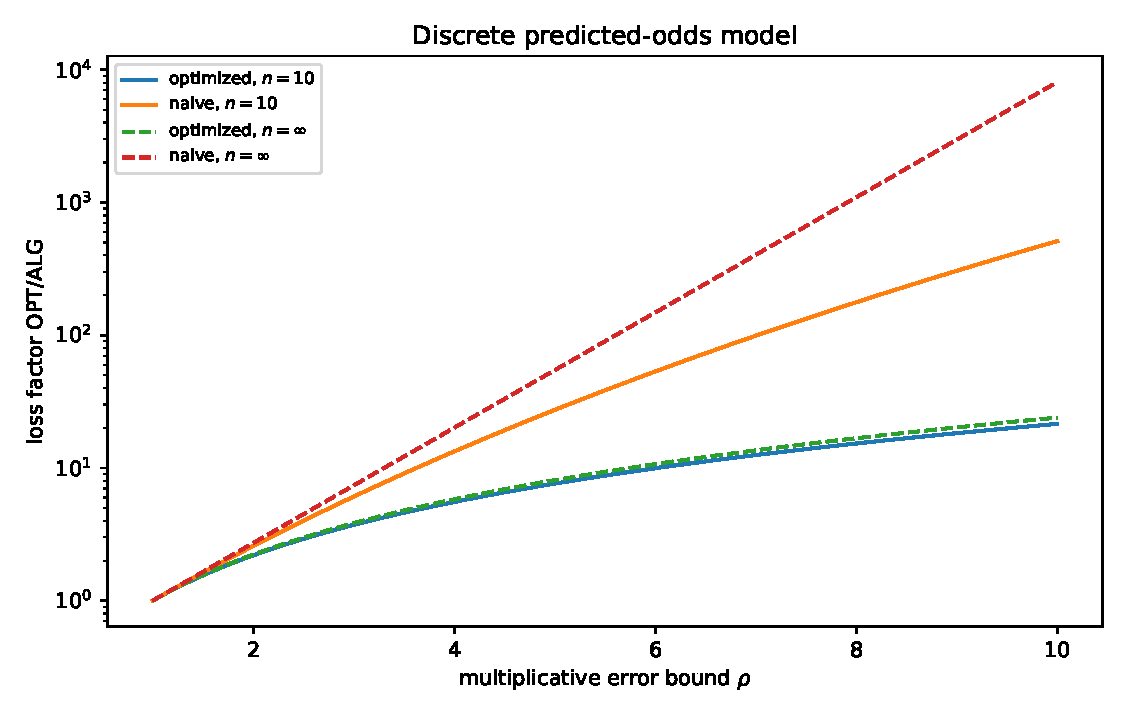
\includegraphics[width=0.95\textwidth]{discrete_ratios.pdf}
\caption{Discrete independent case.  The naive curve is the robust loss of the
fixed nominal target \(\theta=1\); the optimized curve is the
robust-design loss obtained by choosing \(\theta_n^\star(\rho)\) when the error
bound is known.  Both curves report loss factor \(\opt/\alg\).}
\label{fig:discrete-ratios}
\end{figure}

The deterministic minimax theory is therefore complete in the global
worst-case sense: the threshold family yields the exact robust loss curve, and
the optimized target is optimal among all deterministic stopping rules.  The
next section explains why this should not be confused with randomized minimax
optimality.

\section{Beyond deterministic rules}
\label{sec:beyond-deterministic}

\subsection{A two-period randomized minimax example}

The optimized target \(\theta_n^\star(\rho)\) in
Corollary~\ref{cor:optimized-threshold} is deterministic minimax in the global
worst-case sense, by Theorem~\ref{thm:deterministic-minimax}.  It is not,
however, a minimax rule over randomized stopping rules.  This distinction does
not contradict Bruss' theorem: for a fixed known instance, randomization cannot
beat the Bruss optimum, since a randomized rule is a mixture of deterministic
rules.  However, in the robust problem the objective is a worst-case loss factor
over an uncertainty set, and randomization can improve that factor.

The following two-period example makes the point explicit.

\begin{proposition}[A two-period randomized minimax example]
\label{prop:n2-randomized}
Let
\[
  n=2,
  \qquad
  \bar r_1=\bar r_2=1,
  \qquad
  \rho=2.
\]
The best undominated randomized stopping rule has worst-case loss factor
\[
  \boxed{\frac{11}{9}}.
\]
The best deterministic threshold rule has worst-case loss factor \(3/2\).  Hence
randomization is strictly better in this robust minimax sense.
\end{proposition}

\begin{proof}
The multiplicative constraint gives
\[
  r_1,r_2\in\left[\frac12,2\right].
\]
Call a randomized rule dominated if another rule has at least as large a success
probability for every \((r_1,r_2)\in[1/2,2]^2\) and a strictly larger success
probability for some admissible instance.  For a two-period problem, stopping on
a failure is dominated, and failing to stop at time \(2\) after observing a
success is also dominated.  Thus an undominated randomized rule has only one
nontrivial decision: when \(I_1=1\), it stops with some probability
\(a\in[0,1]\).  If it reaches time \(2\), it stops whenever \(I_2=1\).

For \(i=1,2\), write
\[
  p_i=\frac{r_i}{1+r_i},
  \qquad
  q_i=\frac1{1+r_i}.
\]
The rule's success probability is
\[
  W_a(r_1,r_2)
  = a p_1q_2 + q_1p_2 + (1-a)p_1p_2
  = p_2 + a p_1(q_2-p_2).
\]
The clairvoyant Bruss value is
\[
  V^\star(r_1,r_2)
  =
  \begin{cases}
    p_2, & r_2\ge1,\\[0.3em]
    q_1q_2(r_1+r_2), & r_2<1.
  \end{cases}
\]

First suppose that \(r_2\ge1\).  Then
\[
  \frac{W_a}{V^\star}
  =
  1-a\frac{r_1(r_2-1)}{(1+r_1)r_2}.
\]
The subtracted factor is increasing in both \(r_1\) and \(r_2\), so the worst
case on \([1/2,2]^2\cap\{r_2\ge1\}\) is attained at
\(r_1=r_2=2\).  This gives
\[
  \frac{W_a}{V^\star}
  \ge
  1-\frac a3.
\]

Now suppose that \(r_2<1\).  Then
\[
  \frac{W_a}{V^\star}
  =
  \frac{r_2+r_1r_2+a r_1(1-r_2)}{r_1+r_2}.
\]
For fixed \(r_2<1\), this expression is nonincreasing in \(r_1\), hence its
minimum is attained at \(r_1=2\).  With \(r_1=2\), it becomes
\[
  \frac{2a+r_2(3-2a)}{2+r_2},
\]
which is nondecreasing in \(r_2\).  Hence the worst case in the region
\(r_2<1\) is attained at \(r_2=1/2\), and gives
\[
  \frac{W_a}{V^\star}
  \ge
  \frac{2a+3}{5}.
\]
Both lower bounds on \(W_a/V^\star\) are tight, being attained at admissible
endpoints.  Therefore the corresponding loss factor is
\[
  \Delta(a)
  =
  \max\left\{\frac{1}{1-a/3},\frac{5}{2a+3}\right\}.
\]
The first loss-factor term is increasing in \(a\), and the second is decreasing
in \(a\), so the minimum of their maximum is obtained by equalizing the
underlying lower bounds on \(W_a/V^\star\):
\[
  1-\frac a3=\frac{2a+3}{5}.
\]
This yields \(a^\star=6/11\).  The common value of \(W_a/V^\star\) is \(9/11\),
hence the
loss factor is \(11/9\).  The deterministic choices \(a=0\) and \(a=1\) give
loss factors \(5/3\) and \(3/2\), respectively.  Figure~\ref{fig:minimax-n2}
shows the balancing calculation.
\end{proof}

\begin{figure}[ht]
\centering
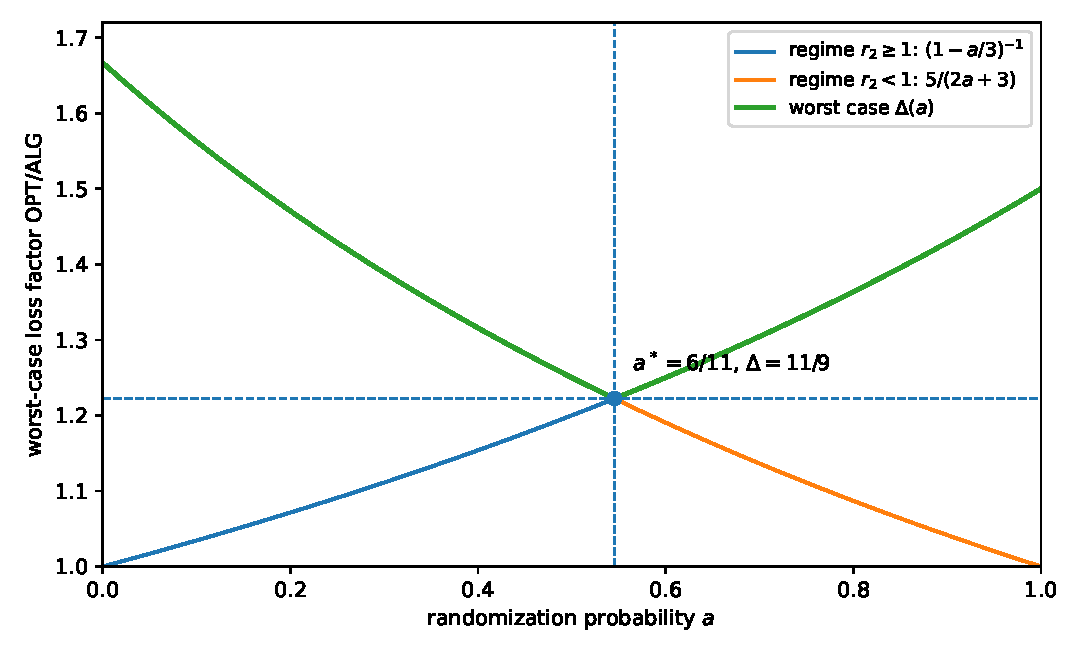
\includegraphics[width=0.85\textwidth]{minimax_n2.pdf}
\caption{The two-period robust example of Proposition~\ref{prop:n2-randomized}.
Among undominated randomized rules, the probability \(a^\star=6/11\) balances
the two adversarial regimes and gives worst-case loss factor \(11/9\).}
\label{fig:minimax-n2}
\end{figure}

\subsection{Exact randomized minimax formulation}

For general \(n\), one should not expect a closed-form minimax randomized rule
of the same simplicity as Bruss' threshold.  Nevertheless, the exact robust
randomized problem has a clean finite-dimensional/semi-infinite formulation.
Let
\[
  \mathcal U
  =
  \prod_{i=1}^n
  \left[\frac{\bar r_i}{\rho},\rho\bar r_i\right]
\]
be the uncertainty set for the true odds.  For a true instance
\(r=(r_1,\dots,r_n)\), define the value of the deterministic threshold \(s\) by
\[
  V_s(r)
  =
  \left(\prod_{j=s}^n\frac1{1+r_j}\right)
  \left(\sum_{j=s}^n r_j\right).
\]
By Bruss' theorem,
\[
  V^\star(r)=\max_{1\le s\le n}V_s(r).
\]

Let \(\mathcal D_n\) be the finite set of deterministic stopping rules on the
binary tree of histories.  For \(d\in\mathcal D_n\), let \(W_d(r)\) be the
probability that rule \(d\) stops on the last success under true odds \(r\).  A
mixed randomized rule is a distribution \(z\in\Delta(\mathcal D_n)\).  Its value
on instance \(r\) is
\[
  W_z(r)=\sum_{d\in\mathcal D_n}z_d W_d(r).
\]
Thus the exact randomized minimax loss factor is
\[
  \Delta_n^\star
  =
  \min_{z\in\Delta(\mathcal D_n)}
  \sup_{r\in\mathcal U}
  \frac{V^\star(r)}{W_z(r)}.
\]
Equivalently, \(\Delta_n^\star\) is the value of the semi-infinite linear program
\[
\begin{aligned}
  \text{minimize}\quad & \sum_{d\in\mathcal D_n} y_d \\
  \text{over}\quad & y_d\ge0 \quad(d\in\mathcal D_n) \\
  \text{subject to}\quad
  & \sum_{d\in\mathcal D_n}y_d W_d(r)
    \ge V_s(r),
    \\
  & \hspace{5em}\forall r\in\mathcal U,
    \quad \forall s\in\{1,\dots,n\}.
\end{aligned}
\]
Indeed, the constraints for all \(s\) are equivalent to
\[
  \sum_{d\in\mathcal D_n}y_d W_d(r)
  \ge
  \max_s V_s(r)
  =
  V^\star(r)
  \qquad
  \forall r\in\mathcal U.
\]
If \(\eta=\sum_d y_d\) and \(\eta>0\), then \(z_d=y_d/\eta\) is a randomized
rule satisfying \(V^\star(r)/W_z(r)\le\eta\) for all \(r\).  Conversely, any
randomized rule with loss factor at most \(\eta\) gives a feasible point
\(y_d=\eta z_d\).


\section{Bayesian calibration under random odds errors}
\label{sec:bayes-random-errors}

The preceding sections treated a worst-case multiplicative uncertainty set.  We
now consider a different, genuinely Bayesian, model.  The odds error is no
longer bounded by a known factor and chosen adversarially.  Instead, each local
multiplicative error is drawn independently from a known law.  The result in this
section is deliberately a reduction rather than a new stopping theorem: after
integrating out the local errors, the indicators are independent with calibrated
success probabilities, so Bruss' theorem applies directly.

\subsection{Independent local multiplicative errors}

The independent-error model is the following.  We observe nominal odds
\[
  \bar r_1,\dots,\bar r_n>0.
\]
For each time $i$, a hidden multiplicative error $\rho_i$ is drawn independently
from a known probability law $\mathcal R$ on $(0,\infty)$, and the true odd is
\[
  \boxed{
  r_i=\frac{\bar r_i}{\rho_i}.
  }
  \tag{12}
\]
Equivalently, the nominal odd is
\[
  \bar r_i=r_i\rho_i.
\]
Conditionally on $\rho_i$, the true success probability at time $i$ is therefore
\[
  p_i(\rho_i)
  =\frac{r_i}{1+r_i}
  =\frac{\bar r_i/\rho_i}{1+\bar r_i/\rho_i}
  =\frac{\bar r_i}{\rho_i+\bar r_i}.
\]
The indicators $I_1,\dots,I_n$ are generated independently conditionally on the
hidden errors $\rho_1,
\dots,\rho_n$.

The objective is the Bayesian one: maximize the conditional, ex ante probability
of stopping on the last success given the observed nominal odds
$\bar r_1,
\dots,\bar r_n$ and the known error law $\mathcal R$.

\begin{remark}[Local errors versus a global error]
This section uses independent local errors $\rho_i$.  This assumption is crucial.
If instead a single unknown factor $\rho$ were shared by all times, then the
observed successes and failures would update the posterior distribution of
$\rho$, and the problem would become a dynamic program on that posterior.  The
simple reduction below would no longer apply.
\end{remark}

\subsection{Marginal independence and effective odds}

Define the Bayesian marginal probability of success at time $i$ by
\[
  \pi_i
  =\mathbb E_{\rho\sim\mathcal R}
  \left[
    \frac{\bar r_i}{\rho+\bar r_i}
  \right].
\]
Then
\[
  1-\pi_i
  =\mathbb E_{\rho\sim\mathcal R}
  \left[
    \frac{\rho}{\rho+\bar r_i}
  \right].
\]
The corresponding Bayesian effective odd is
\[
  \boxed{
  b_i
  :=\frac{\pi_i}{1-\pi_i}
  =
  \frac{
    \mathbb E_{\rho\sim\mathcal R}
    \left[\dfrac{\bar r_i}{\rho+\bar r_i}\right]
  }{
    \mathbb E_{\rho\sim\mathcal R}
    \left[\dfrac{\rho}{\rho+\bar r_i}\right]
  }.
  }
  \tag{13}
\]

\begin{lemma}[Marginal independence after integrating the local errors]
\label{lem:marginal-independence}
Under the independent-error model, conditional on the nominal odds $\bar r_1,
\dots,\bar r_n$, the
indicators $I_1,\dots,I_n$ are independent Bernoulli random variables with
success probabilities $\pi_1,
\dots,\pi_n$.
\end{lemma}

\begin{proof}
Fix a vector $\varepsilon=(\varepsilon_1,
\dots,\varepsilon_n)\in\{0,1\}^n$.
Conditionally on the hidden errors, the indicators are independent, hence
\[
  \mathbb P(I_1=\varepsilon_1,
\dots,I_n=\varepsilon_n\mid \rho_1,
\dots,\rho_n)
  =
  \prod_{i=1}^n
  p_i(\rho_i)^{\varepsilon_i}
  \bigl(1-p_i(\rho_i)\bigr)^{1-\varepsilon_i}.
\]
Taking expectation over the independent hidden errors $\rho_i$ factorizes the
right-hand side:
\begin{align*}
  \mathbb P(I_1=\varepsilon_1,
\dots,I_n=\varepsilon_n)
  &=
  \prod_{i=1}^n
  \mathbb E\left[
    p_i(\rho_i)^{\varepsilon_i}
    \bigl(1-p_i(\rho_i)\bigr)^{1-\varepsilon_i}
  \right] \\
  &=
  \prod_{i=1}^n
  \pi_i^{\varepsilon_i}(1-\pi_i)^{1-\varepsilon_i}.
\end{align*}
This is exactly the joint law of independent Bernoulli variables with parameters
$\pi_i$.
\end{proof}

\begin{theorem}[Bayesian odds theorem under independent local errors]
\label{thm:bayes-bruss}
Under the independent-error model, the Bayesian optimal rule is obtained by
applying Bruss' odds algorithm to the effective odds \(b_i\) defined in
\((13)\).  That is, define
\[
  B_k=\sum_{j=k}^n b_j,
  \qquad
  \widetilde Q_k=\prod_{j=k}^n(1-\pi_j),
\]
with $B_{n+1}=0$.  In the non-degenerate case $B_1>1$, let
\[
  s_{\mathcal R}
  =\sup\left\{k:B_k\ge1\right\}.
\]
Then the Bayesian optimal rule ignores successes before $s_{\mathcal R}$ and
stops at the first success from $s_{\mathcal R}$ onward.  Its Bayesian value is
\[
  \boxed{
  V_{\mathcal R}^{\star}
  =\widetilde Q_{s_{\mathcal R}}B_{s_{\mathcal R}}.
  }
  \tag{14}
\]
If $B_1<1$, the Bayesian optimal rule stops at the first success from the
beginning.  If $B_1=1$, the same start-at-\(1\) rule is optimal, with value
\(\widetilde Q_1B_1\).
\end{theorem}

\begin{proof}
By Lemma~\ref{lem:marginal-independence}, after the hidden local errors have
been integrated out, the Bayesian problem conditional on the nominal odds is an
ordinary independent Bernoulli last-success problem with success probabilities
$\pi_i$.  Its odds are precisely
\[
  \frac{\pi_i}{1-\pi_i}=b_i.
\]
Bruss' odds theorem therefore applies verbatim to the sequence
$\pi_1,
\dots,\pi_n$.  It says to sum the odds $b_i$ from the end until reaching one,
and then stop at the first success from that index onward.  The value formula is
the usual threshold value formula
\[
  \left(\prod_{j=s_{\mathcal R}}^n(1-\pi_j)\right)
  \left(\sum_{j=s_{\mathcal R}}^n b_j\right)
  =\widetilde Q_{s_{\mathcal R}}B_{s_{\mathcal R}}.
\]
This proves the claim.
\end{proof}

\subsection{The calibration map}

It is useful to view the theorem as a deterministic calibration of the nominal
odds.  For $x>0$, define
\[
  M_{\mathcal R}(x)
  =\mathbb E_{\rho\sim\mathcal R}\left[\frac1{\rho+x}\right].
\]
Then
\[
  \pi(x)=xM_{\mathcal R}(x),
  \qquad
  1-\pi(x)=1-xM_{\mathcal R}(x),
\]
and the effective odd associated with a nominal odd $x$ is
\[
  \boxed{
  B_{\mathcal R}(x)
  =\frac{xM_{\mathcal R}(x)}{1-xM_{\mathcal R}(x)}.
  }
  \tag{15}
\]
Thus the independent-error model is algorithmically simple:
\[
  \boxed{
  \bar r_i\quad\longmapsto\quad B_{\mathcal R}(\bar r_i),
  \quad\text{then apply Bruss to these calibrated odds.}
  }
\]

\begin{lemma}[Basic properties of the calibration map]
\label{lem:calibration-properties}
For any law $\mathcal R$ on $(0,\infty)$, the map
$x\mapsto B_{\mathcal R}(x)$ is nondecreasing and finite for every $x>0$.
Moreover, if $\mathbb E[1/\rho]<\infty$, then
\[
  B_{\mathcal R}(x)
  \sim x\mathbb E\left[\frac1\rho\right]
  \qquad (x\downarrow0),
\]
and if $\mathbb E[\rho]<\infty$, then
\[
  B_{\mathcal R}(x)
  \sim \frac{x}{\mathbb E[\rho]}
  \qquad (x\to\infty).
\]
\end{lemma}

\begin{proof}
The function $x\mapsto x/(\rho+x)$ is increasing for every fixed $\rho>0$.
Therefore
\[
  \pi(x)=\mathbb E\left[\frac{x}{\rho+x}\right]
\]
is nondecreasing.  Since $0<x/(\rho+x)<1$ for every $\rho>0$, one has
$0<\pi(x)<1$, hence
\[
  B_{\mathcal R}(x)=\frac{\pi(x)}{1-\pi(x)}
\]
is finite and nondecreasing.

If $\mathbb E[1/\rho]<\infty$, then
\[
  \frac1x\pi(x)
  =\mathbb E\left[\frac1{\rho+x}\right]
  \longrightarrow
  \mathbb E\left[\frac1\rho\right]
\]
by monotone convergence.  Since $\pi(x)\to0$ as $x\downarrow0$, this gives
$B_{\mathcal R}(x)\sim \pi(x)\sim x\mathbb E[1/\rho]$.

If $\mathbb E[\rho]<\infty$, write
\[
  1-\pi(x)=\mathbb E\left[\frac{\rho}{\rho+x}\right].
\]
Then
\[
  x(1-\pi(x))
  =\mathbb E\left[\frac{x\rho}{\rho+x}\right]
  \longrightarrow
  \mathbb E[\rho]
\]
by monotone convergence, because $x\rho/(x+\rho)\uparrow\rho$.  Since
$\pi(x)\to1$, we obtain
\[
  B_{\mathcal R}(x)
  =\frac{\pi(x)}{1-\pi(x)}
  \sim \frac1{1-\pi(x)}
  \sim \frac{x}{\mathbb E[\rho]}.
\]
\end{proof}

\subsection{Examples of error laws}

The only quantity needed by the algorithm is $M_{\mathcal R}(x)$.  For several
simple laws it is explicit.

\paragraph{Deterministic multiplicative error.}
If $\rho\equiv c$, then
\[
  M_{\mathcal R}(x)=\frac1{c+x},
  \qquad
  B_{\mathcal R}(x)=\frac{x}{c}.
\]
This recovers the obvious rescaling of all nominal odds.

\paragraph{Finite mixture.}
If $\rho=c_\ell$ with probability $w_\ell$, where $\sum_\ell w_\ell=1$, then
\[
  M_{\mathcal R}(x)=\sum_\ell\frac{w_\ell}{c_\ell+x},
\]
and therefore
\[
  B_{\mathcal R}(x)
  =
  \frac{
    x\sum_\ell\dfrac{w_\ell}{c_\ell+x}
  }{
    1-x\sum_\ell\dfrac{w_\ell}{c_\ell+x}
  }.
\]
This is often the most practical case numerically: a continuous law can be
approximated by a finite mixture, after which the algorithm is fully explicit.

\paragraph{Uniform law.}
If $\rho\sim\mathrm{Unif}[a,b]$, with $0<a<b$, then
\[
  M_{\mathcal R}(x)
  =\frac1{b-a}\log\left(\frac{b+x}{a+x}\right),
\]
so
\[
  B_{\mathcal R}(x)
  =
  \frac{
    \dfrac{x}{b-a}\log\left(\dfrac{b+x}{a+x}\right)
  }{
    1-\dfrac{x}{b-a}\log\left(\dfrac{b+x}{a+x}\right)
  }.
\]

\paragraph{Gamma law.}
Let $\rho\sim\Gamma(a,\beta)$, where $a>0$ is the shape and $\beta>0$ is the rate:
\[
  f(\rho)=\frac{\beta^a}{\Gamma(a)}\rho^{a-1}e^{-\beta\rho},
  \qquad \rho>0.
\]
Then
\[
  \boxed{
  M_{\mathcal R}(x)
  =
  \beta^a x^{a-1}e^{\beta x}\Gamma(1-a,\beta x),
  }
  \tag{16}
\]
where $\Gamma(\cdot,\cdot)$ denotes the upper incomplete gamma function.  Hence
\[
  \boxed{
  B_{\mathcal R}(x)
  =
  \frac{
    \beta^a x^a e^{\beta x}\Gamma(1-a,\beta x)
  }{
    1-\beta^a x^a e^{\beta x}\Gamma(1-a,\beta x)
  }.
  }
  \tag{17}
\]
For the exponential case $a=1$, this becomes
\[
  M_{\mathcal R}(x)=\beta e^{\beta x}E_1(\beta x),
\]
where
\[
  E_1(y)=\int_y^\infty\frac{e^{-t}}{t}\,dt.
\]

\paragraph{Shifted half-normal law.}
If
\[
  \rho=1+|Z|,
  \qquad
  Z\sim\mathcal N(0,\sigma^2),
\]
then $\rho\ge1$, so the nominal odds always overestimate the true odds.  In this
case
\[
  \boxed{
  M_{\mathcal R}(x)
  =
  \sqrt{\frac\pi2}\frac1\sigma
  \exp\left(\frac{(x+1)^2}{2\sigma^2}\right)
  \operatorname{erfc}\left(\frac{x+1}{\sqrt2\sigma}\right).
  }
  \tag{18}
\]
Again $B_{\mathcal R}(x)=xM_{\mathcal R}(x)/(1-xM_{\mathcal R}(x))$.

The table and Figure~\ref{fig:bayes-calibration} illustrate the resulting
calibration maps.
In the table, \(x\) is a possible observed nominal odd, \(x=\bar r_i\).  Each
entry is the calibrated effective odd \(B_{\mathcal R}(x)\) that should replace
\(\bar r_i\) before summing odds.

\begin{table}[ht]
\centering
\caption{Examples of the Bayesian calibration $x=\bar r\mapsto B_{\mathcal R}(x)$.
Rows are nominal odds \(x\), and entries are calibrated effective odds.  The
exponential law has mean $1$ but large variance and mass near $0$, which inflates
small effective odds.  The shifted half-normal law satisfies $\rho\ge1$, hence it
mostly deflates the nominal odds.}
\begin{tabular}{c c c c c}
\toprule
nominal odd $x=\bar r_i$ & $\rho\equiv1$ & $\mathrm{Unif}[0.5,1.5]$ & $\mathrm{Exp}(1)$ & $1+|N(0,0.5^2)|$\\
\midrule
0.1 & 0.100 & 0.109 & 0.252 & 0.085\\
0.5 & 0.500 & 0.530 & 0.857 & 0.438\\
1.0 & 1.000 & 1.044 & 1.477 & 0.899\\
2.0 & 2.000 & 2.058 & 2.606 & 1.853\\
5.0 & 5.000 & 5.071 & 5.762 & 4.803\\
\bottomrule
\end{tabular}
\end{table}

\begin{figure}[ht]
\centering
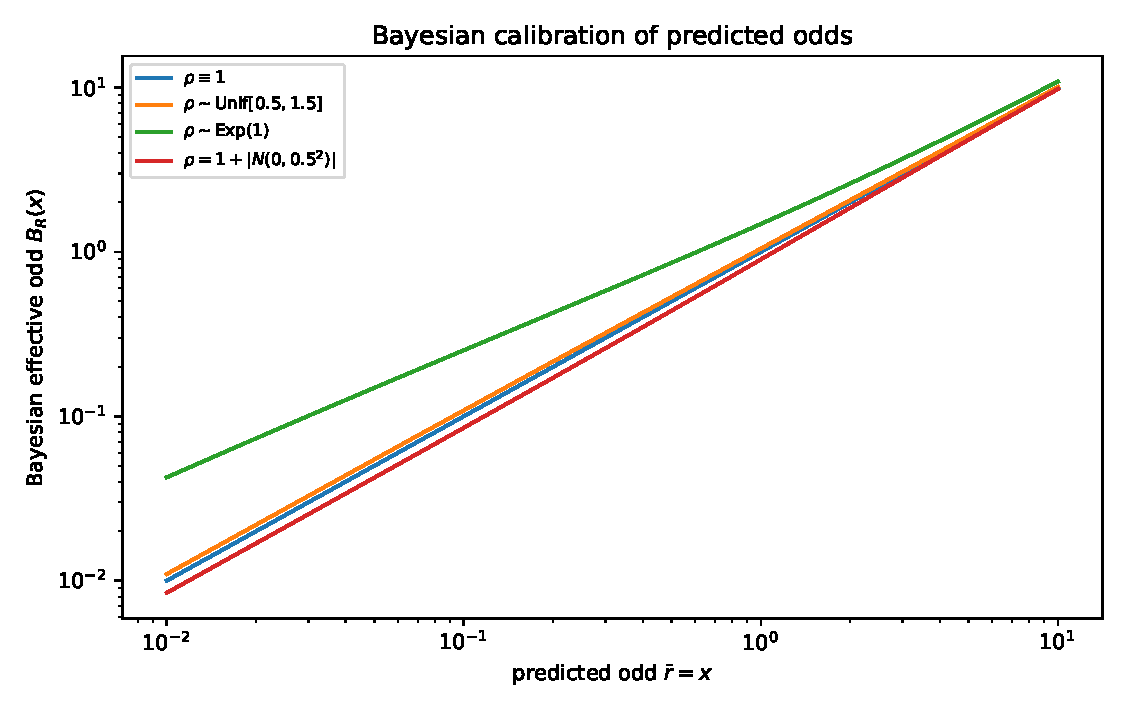
\includegraphics[width=0.95\textwidth]{bayes_calibration.pdf}
\caption{Bayesian calibration map $x\mapsto B_{\mathcal R}(x)$ for several
independent local error laws.  After calibration, the Bayesian optimal algorithm
is Bruss' odds rule applied to the transformed odds.}
\label{fig:bayes-calibration}
\end{figure}

\subsection{Worst-case robustness versus Bayesian calibration}

The worst-case robust model asks for a threshold that performs well for every
realization of the multiplicative error up to a factor \(\rho\).  The
independent-error model asks a different question: if the local errors are
random with known law, what rule maximizes the Bayesian success probability?
The answer is especially neat:
there is no need for a new stopping theorem.  Random local multiplicative errors
only change the Bernoulli probabilities.  Once those induced probabilities are
computed, Bruss' theorem applies without modification.

In short,
\[
  \boxed{
  \text{random independent local errors }
  \Longrightarrow
  \text{calibrate odds, then sum calibrated odds to one.}
  }
\]

The next section returns from Bayesian calibration to worst-case robustness, but
in a continuous arrival model where the relevant state is a remaining intensity
mass rather than a finite tail sum of odds.

\section{Continuous Poisson model}
\label{sec:poisson}

We now pass from a finite Bernoulli sequence to a continuous-time arrival
model.  The state variable becomes the remaining intensity mass, and a nominal
target chooses when that remaining nominal mass reaches a prescribed level.

Let successes arrive on
\([0,T]\) according to an inhomogeneous Poisson process with true intensity
\(\varphi(t)\).  Define the true remaining mass
\[
  M(t)=\int_t^T\varphi(u)\,du.
\]
If we start accepting at time \(t\) and then stop at the first success after
\(t\), we win if and only if there is exactly one success after \(t\).  Since the
number of future successes is Poisson with mean \(M(t)\),
\[
  W(t)=\mathbb P(\Pois(M(t))=1)=M(t)\e^{-M(t)}.
\]
The function \(m\mapsto m\e^{-m}\) is maximized at \(m=1\), with value \(1/\e\).
Thus, when the known total future mass satisfies \(M(0)\ge1\), the optimal rule
is
\[
  \boxed{
  \int_\tau^T\varphi(u)\,du=1,
  \quad\text{then stop at the first success after }\tau.
  }
  \tag{8}
\]
If \(M(0)<1\), the level \(1\) is not reachable and the optimal rule starts
immediately at time \(0\), with value \(M(0)\e^{-M(0)}\).  In the robust
calibration below, \(1/\e\) is the interior benchmark; when the total true mass
does not reach one, it remains a universal upper bound rather than the attained
optimal value.

\subsection{Robust nominal intensity}

Suppose now that only a nominal intensity \(\bar\varphi(t)\) is known, and that
\[
  \boxed{
  \frac1\rho\bar\varphi(t)\le\varphi(t)\le\rho\bar\varphi(t)
  }
  \qquad\text{for every }t\in[0,T].
  \tag{B}
\]
Let
\[
  \bar M(t)=\int_t^T\bar\varphi(u)\,du.
\]
A target \(\theta\) means choosing \(\tau_\theta\) such that
\[
  \bar M(\tau_\theta)=\theta,
\]
and then stopping at the first success after \(\tau_\theta\).  Since
\(\bar M\) is absolutely continuous and nonincreasing, this crossing exists
whenever the nominal total mass satisfies \(\bar M(0)\ge\theta\).  By \((B)\),
the true remaining mass satisfies
\[
  M(\tau_\theta)\in\left[\frac{\theta}{\rho},\rho\theta\right].
\]
Against the interior benchmark \(1/\e\), the guaranteed loss factor of target
\(\theta\) is
\[
  \frac{1/\e}{\min_{m\in[\theta/\rho,\rho\theta]}m\e^{-m}}.
\]
This is an interior, target-reachable calibration problem: it assumes the
nominal mass is large enough to reach the chosen target and compares against
the \(1/\e\) benchmark that is attainable when the true total mass reaches one.
Boundary cases are discussed after the theorem.

\begin{theorem}[Optimal interior robust Poisson target]
\label{thm:poisson-robust}
For \(\rho>1\), the target that optimizes the interior robust-calibration problem
against the \(1/\e\) benchmark is
\[
  \boxed{
  \theta^\star_{\mathrm P}(\rho)
  =
  \frac{2\rho\log\rho}{\rho^2-1}.
  }
  \tag{9}
\]
The continuous extension gives \(\theta^\star_{\mathrm P}(1)=1\).  The resulting
worst-case loss factor against the interior \(1/\e\) benchmark is
\[
  \boxed{
  \Lambda_{\mathrm P}(\rho)
  =
  \frac{\rho^2-1}{2\log\rho}
  \exp\left(\frac{2\log\rho}{\rho^2-1}-1\right).
  }
  \tag{10}
\]
\end{theorem}

\begin{proof}
Let
\[
  f(m)=m\e^{-m}.
\]
Then \(f\) is strictly increasing on \((0,1)\), strictly decreasing on
\((1,\infty)\), and maximized at \(m=1\).

For a fixed target \(\theta\), the uncertainty interval for the true mass is
\([\theta/\rho,\rho\theta]\).  The robust value before multiplying by \(\e\) is
\[
  \min_{m\in[\theta/\rho,\rho\theta]}f(m).
\]
We consider three possible regimes.

\medskip
\noindent\emph{Regime 1: \(\rho\theta\le1\).}
Then the whole interval lies to the left of the maximizer.  Since \(f\) is
increasing on \((0,1)\), the minimum is \(f(\theta/\rho)\).  Increasing
\(\theta\) increases this value while preserving \(\rho\theta\le1\) until
\(\rho\theta=1\).

\medskip
\noindent\emph{Regime 2: \(\theta/\rho\ge1\).}
Then the whole interval lies to the right of the maximizer.  Since \(f\) is
decreasing on \((1,\infty)\), the minimum is \(f(\rho\theta)\).  Decreasing
\(\theta\) increases this value while preserving \(\theta/\rho\ge1\) until
\(\theta/\rho=1\).

\medskip
\noindent\emph{Regime 3: \(\theta/\rho<1<\rho\theta\).}
Then the minimum is
\[
  \min\left\{f\left(\frac{\theta}{\rho}\right),f(\rho\theta)\right\}.
\]
As \(\theta\) increases inside this regime,
\(f(\theta/\rho)\) increases and \(f(\rho\theta)\) decreases.  Hence the
max-min point is where the two endpoint values are equal:
\[
  f\left(\frac{\theta}{\rho}\right)=f(\rho\theta).
\]
This is
\[
  \frac{\theta}{\rho}\e^{-\theta/\rho}
  =
  \rho\theta\e^{-\rho\theta}.
\]
Since \(\theta>0\), cancellation gives
\[
  1=\rho^2\e^{-(\rho-1/\rho)\theta}.
\]
Taking logarithms yields
\[
  \theta^\star_{\mathrm P}
  =\frac{2\rho\log\rho}{\rho^2-1}.
\]

It remains only to check that this point indeed lies in Regime 3.  We need
\[
  \frac1\rho<\theta^\star_{\mathrm P}<\rho.
\]
The upper bound is equivalent to
\[
  2\log\rho<\rho^2-1,
\]
which holds strictly for \(\rho>1\).  The lower bound is equivalent to
\[
  \rho^2\log(\rho^2)>\rho^2-1,
\]
or, with \(y=\rho^2>1\),
\[
  y\log y>y-1,
\]
which also holds for \(y>1\).  Thus the equalizing point is feasible and it
beats the boundary optima of the other regimes.

Finally, at the optimum the worst endpoint is
\[
  \frac{\theta^\star_{\mathrm P}}{\rho}
  =
  \frac{2\log\rho}{\rho^2-1}.
\]
The guaranteed probability is
\((\theta^\star_{\mathrm P}/\rho)\e^{-\theta^\star_{\mathrm P}/\rho}\), and the
loss factor against the interior benchmark \(1/\e\) is
\[
  \frac{1/\e}
  {(\theta^\star_{\mathrm P}/\rho)\e^{-\theta^\star_{\mathrm P}/\rho}}
  =
  \frac{\rho}{\theta^\star_{\mathrm P}}
  \exp\left(\frac{\theta^\star_{\mathrm P}}{\rho}-1\right),
\]
which is exactly \((10)\).
\end{proof}

\begin{remark}[Boundary nominal-mass case]
If \(\bar M(0)<\theta\), the target level is not reachable.  The natural
boundary convention is then to start immediately at time \(0\).  This case has
success probability \(M(0)\e^{-M(0)}\), where
\[
  M(0)\in\left[\frac{\bar M(0)}{\rho},\rho\bar M(0)\right].
\]
There is no nontrivial lower bound depending only on the chosen target
\(\theta\), because the total nominal mass \(\bar M(0)\) may be arbitrarily
small.  Thus Theorem~\ref{thm:poisson-robust} is not a global theorem over all
possible boundary masses.  It is the interior robust-calibration statement: it
applies to instances with enough nominal remaining mass to reach the optimized
target and uses \(1/\e\) as the reachable interior benchmark.  Boundary starts
are handled by the immediate-start convention rather than by a different
calibrated threshold.
\end{remark}

\subsection{Naive Poisson target}

The naive rule targets \(\bar M(t)=1\).  Then the true remaining mass lies in
\[
  \left[\frac1\rho,\rho\right].
\]
The guaranteed loss factor is therefore
\[
  \boxed{
  B_{\mathrm P}(\rho)
  =
  \max\left\{
    \rho\exp\left(\frac1\rho-1\right),
    \frac1\rho\e^{\rho-1}
  \right\}.
  }
  \tag{11}
\]
The optimized robust target satisfies
\[
  \theta^\star_{\mathrm P}(\rho)<1
  \qquad(\rho>1),
\]
so, as in the discrete case, robustness means starting slightly later than the
naive nominal target.  Figure~\ref{fig:poisson-ratios} compares the
corresponding loss factors, while Figure~\ref{fig:target-levels} compares the
optimized target levels.

\begin{table}[ht]
\centering
\caption{Continuous Poisson model.  Interior optimized robust calibration versus
the naive target.  As \(\rho\) grows, the optimized target equalizes the endpoint
success probabilities and avoids the exponential deterioration of the naive loss
factor.}
\begin{tabular}{c c c c}
\toprule
\(\rho\)
& \(\theta^\star_{\mathrm P}\)
& \(\Lambda_{\mathrm P}\)
& \(B_{\mathrm P}\)\\
\midrule
1 & 1.000 & 1.000 & 1.000 \\
1.25 & 0.992 & 1.025 & 1.027 \\
1.5 & 0.973 & 1.085 & 1.099 \\
2 & 0.924 & 1.264 & 1.359 \\
3 & 0.824 & 1.763 & 2.463 \\
5 & 0.671 & 3.137 & 10.920 \\
10 & 0.465 & 8.285 & 810.308 \\
\bottomrule
\end{tabular}
\end{table}

\begin{figure}[ht]
\centering
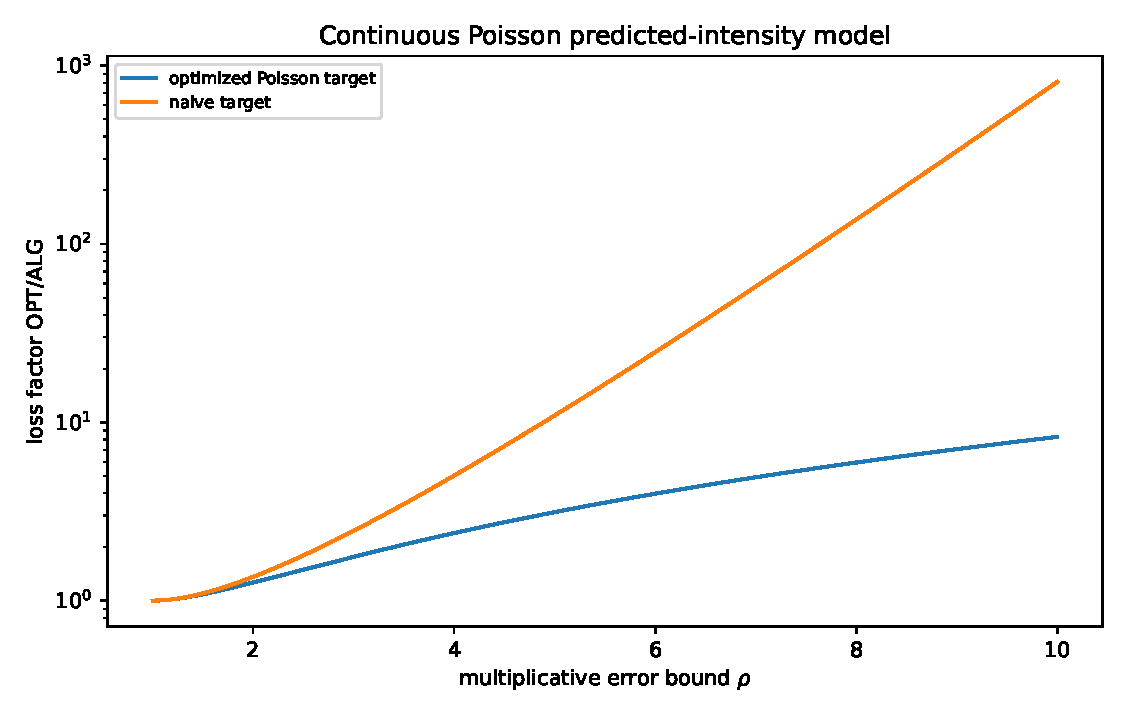
\includegraphics[width=0.95\textwidth]{poisson_ratios.pdf}
\caption{Continuous Poisson case.  The optimized curve is for the interior
target-reachable robust calibration problem against the \(1/\e\) benchmark.  The
optimized target equalizes the two endpoint success probabilities at masses
\(\theta/\rho\) and \(\rho\theta\).}
\label{fig:poisson-ratios}
\end{figure}

\begin{figure}[ht]
\centering
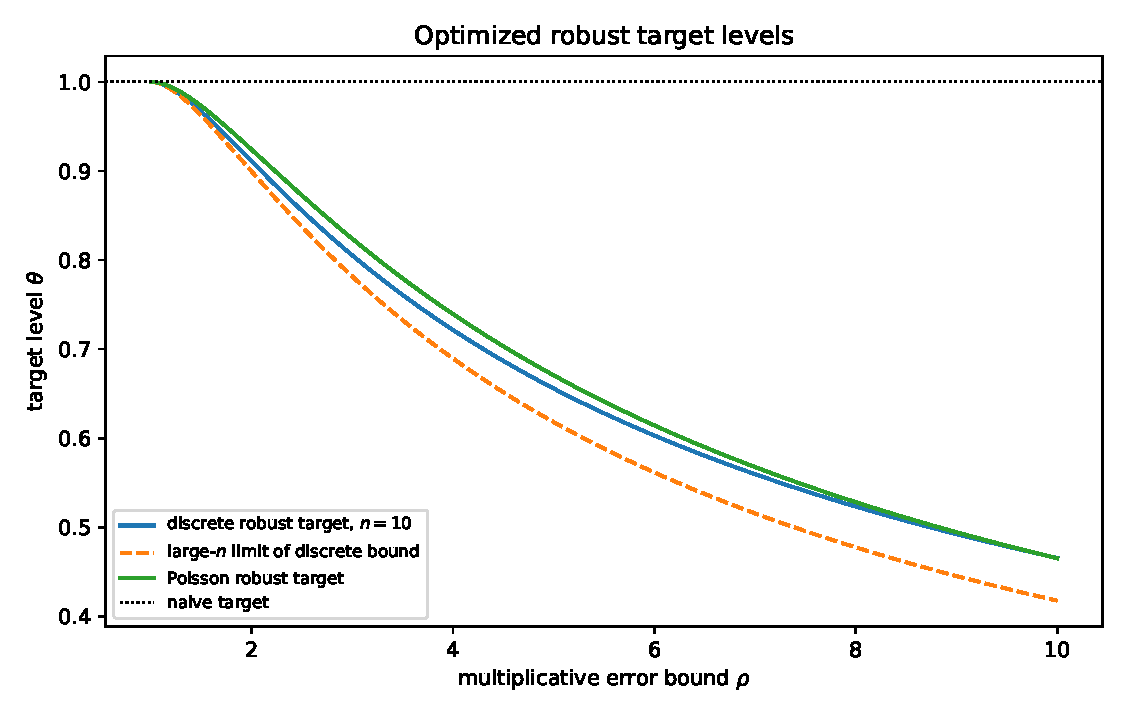
\includegraphics[width=0.95\textwidth]{targets.pdf}
\caption{Optimized target levels for the discrete robust-design rule, its
large-\(n\) limiting curve, and the interior Poisson calibration.  The plotted
targets are below \(1\) as soon as \(\rho>1\); the finite-\(n\) exception
\(\theta_2^\star(\rho)=1\) is not shown.}
\label{fig:target-levels}
\end{figure}

\begin{remark}[Discrete large-\(n\) bound versus the Poisson target]
The curve labelled as the large-\(n\) limit of the discrete bound in
Figure~\ref{fig:target-levels} should not be read as the Poisson limit of the
stochastic model.  It is the limit of the finite-\(n\) uniform guarantee proved
above.  In the early-start case, that proof uses the bound
\[
  \frac{W_\theta}{V^\star}\ge \exp(1-\rho\theta),
\]
which leads to the equation
\[
  \theta\e^{\rho\theta-1}=\rho.
\]
In the Poisson model the success probability at remaining mass \(m\) is exactly
\(m\e^{-m}\), so the robust target instead equalizes the two endpoint
probabilities
\[
  \frac{\theta}{\rho}\exp\left(-\frac{\theta}{\rho}\right)
  =
  \rho\theta\e^{-\rho\theta}.
\]
This gives \(\theta^\star_{\mathrm P}=2\rho\log\rho/(\rho^2-1)\).  The two curves therefore
need not coincide; the apparent closeness of the Poisson target to the \(n=10\)
curve in the plotted range is a numerical feature of these formulas, not a
convergence statement.
\end{remark}

\section{Conclusion}

This paper revisits Bruss' odds theorem as a robust optimization problem with
nominal odds.  Exact nominal odds recover the classical Bruss threshold.  If the
nominal vector is allowed to be arbitrarily unrelated to the truth, no stopping
rule can improve on the tight \(n\)-loss baseline.  Under coordinatewise
multiplicative odds uncertainty, however, the structure of the odds theorem gives
an exact global finite-\(n\) robust loss curve for every deterministic
nominal-threshold rule and every target \(\theta>0\).  When the uncertainty
radius \(\rho\) is known, the optimized robust target is obtained by balancing
two interpretable risks: starting too late when the true tail is lighter than
the nominal tail, and starting too early when the true tail is heavier.

The results also clarify the scope of this explicit theory.  The optimized
target is deterministic minimax in the global worst-case sense, but the
two-period example shows that randomized minimax rules can do better in some
uncertainty sets.  The Bayesian section answers a different question: when local
multiplicative odds errors are independent and drawn from a known law, the
correct operation is odds calibration followed by Bruss' theorem.  The Poisson
section is an interior continuous calibration analogue, not a boundary-inclusive
robust stopping theorem; in that interior benchmark, the robust target equalizes
endpoint risks.

Several directions are deliberately outside the present scope.  We do not model
how the nominal odds are estimated from data or make empirical claims about a
particular forecasting system.  Bayesian calibration relies on independent local
errors; a shared or dependent error would generally require a posterior-state
dynamic program.  More general robust optimal stopping under ambiguity is also a
different problem.  The point of the present model is that the odds
representation makes robust threshold design explicit: exact recovery when the
nominal odds are correct, a tight unbounded-uncertainty barrier, and global
finite-\(n\) robust loss formulas under multiplicative odds uncertainty.

\appendix

\section{Auxiliary inequalities used in the proofs}

\begin{lemma}[Product dominates one plus the sum]
For nonnegative \(u_1,\dots,u_m\),
\[
  \prod_{i=1}^m(1+u_i)\ge1+\sum_{i=1}^m u_i.
\]
\end{lemma}

\begin{proof}
Expand the product by choosing, for each index \(i\), either the term \(1\) or
the term \(u_i\).  Equivalently,
\[
  \prod_{i=1}^m(1+u_i)
  =
  \sum_{A\subseteq\{1,\dots,m\}}\prod_{i\in A}u_i
  =
  1+\sum_{i=1}^m u_i
  +\sum_{\substack{A\subseteq\{1,\dots,m\}\\ |A|\ge2}}\prod_{i\in A}u_i .
\]
The last sum is nonnegative because all \(u_i\) are nonnegative.  Discarding
these higher-order terms gives the claimed lower bound.
\end{proof}

\begin{lemma}[AM--GM product bound]
If \(z_1,
\dots,z_m\ge0\) and \(z_1+\cdots+z_m\le S\), then
\[
  \prod_{i=1}^m z_i\le\left(\frac{S}{m}\right)^m.
\]
\end{lemma}

\begin{proof}
If one of the \(z_i\)'s is zero, then the left-hand side is zero and the
inequality is immediate.  We may therefore assume \(z_i>0\) for all \(i\).
The arithmetic--geometric mean inequality gives
\[
  \left(\prod_{i=1}^m z_i\right)^{1/m}
  \le
  \frac1m\sum_{i=1}^m z_i
  \le
  \frac{S}{m}.
\]
Both sides are nonnegative, so raising to the power \(m\) preserves the
inequality and yields
\[
  \prod_{i=1}^m z_i\le\left(\frac{S}{m}\right)^m .
\]
\end{proof}

\begin{thebibliography}{99}

\bibitem{ChowRobbinsSiegmund1971}
Yuan Shih Chow, Herbert Robbins, and David Siegmund.
\newblock \emph{Great Expectations: The Theory of Optimal Stopping}.
\newblock Houghton Mifflin, Boston, 1971.

\bibitem{GilbertMosteller1966}
John P. Gilbert and Frederick Mosteller.
\newblock Recognizing the maximum of a sequence.
\newblock \emph{Journal of the American Statistical Association},
61(313):35--73, 1966.
\newblock doi:10.1080/01621459.1966.10502008.

\bibitem{Bruss2000}
F. Thomas Bruss.
\newblock Sum the odds to one and stop.
\newblock \emph{The Annals of Probability}, 28(3):1384--1391, 2000.
\newblock doi:10.1214/aop/1019160340.

\bibitem{Bruss2003}
F. Thomas Bruss.
\newblock A note on bounds for the odds theorem of optimal stopping.
\newblock \emph{The Annals of Probability}, 31(4):1859--1861, 2003.
\newblock doi:10.1214/aop/1068646368.

\bibitem{Bruss2019}
F. Thomas Bruss.
\newblock Odds-theorem and monotonicity.
\newblock \emph{Mathematica Applicanda}, 47(1):25--43, 2019.
\newblock doi:10.14708/ma.v47i1.6481.

\bibitem{BrussPaindaveine2000}
F. Thomas Bruss and Davy Paindaveine.
\newblock Selecting a sequence of last successes in independent trials.
\newblock \emph{Journal of Applied Probability}, 37(2):389--399, 2000.
\newblock doi:10.1239/jap/1014842544.

\bibitem{HsiauYang2002}
Shoou-Ren Hsiau and Jiing-Ru Yang.
\newblock Selecting the last success in Markov-dependent trials.
\newblock \emph{Journal of Applied Probability}, 39(2):271--281, 2002.
\newblock doi:10.1239/jap/1025131425.

\bibitem{BrussLouchard2009}
F. Thomas Bruss and Guy Louchard.
\newblock The odds algorithm based on sequential updating and its performance.
\newblock \emph{Advances in Applied Probability}, 41(1):131--153, 2009.
\newblock doi:10.1239/aap/1240319579.

\bibitem{Ferguson2016}
Thomas S. Ferguson.
\newblock The sum-the-odds theorem with application to a stopping game of
Sakaguchi.
\newblock \emph{Mathematica Applicanda}, 44(1):45--61, 2016.
\newblock doi:10.14708/ma.v44i1.1192.

\bibitem{Tamaki2010}
Mitsushi Tamaki.
\newblock Sum the multiplicative odds to one and stop.
\newblock \emph{Journal of Applied Probability}, 47(3):761--777, 2010.
\newblock doi:10.1239/jap/1285335408.

\bibitem{AnoKakinumaMiyoshi2010}
Katsunori Ano, Hideo Kakinuma, and Naoto Miyoshi.
\newblock Odds theorem with multiple selection chances.
\newblock \emph{Journal of Applied Probability}, 47(4):1093--1104, 2010.
\newblock doi:10.1239/jap/1294170522.

\bibitem{BrussYor2012}
F. Thomas Bruss and Marc Yor.
\newblock Stochastic processes with proportional increments and the
last-arrival problem.
\newblock \emph{Stochastic Processes and their Applications},
122(9):3239--3261, 2012.
\newblock doi:10.1016/j.spa.2012.05.010.

\bibitem{Riedel2009}
Frank Riedel.
\newblock Optimal stopping with multiple priors.
\newblock \emph{Econometrica}, 77(3):857--908, 2009.
\newblock doi:10.3982/ECTA7594.

\bibitem{BayraktarYao2014}
Erhan Bayraktar and Song Yao.
\newblock On the robust optimal stopping problem.
\newblock \emph{SIAM Journal on Control and Optimization},
52(5):3135--3175, 2014.
\newblock doi:10.1137/130950331.

\bibitem{MitzenmacherVassilvitskii2020}
Michael Mitzenmacher and Sergei Vassilvitskii.
\newblock Algorithms with predictions.
\newblock arXiv:2006.09123, 2020.
\newblock doi:10.48550/arXiv.2006.09123.

\bibitem{LykourisVassilvitskii2018}
Thodoris Lykouris and Sergei Vassilvitskii.
\newblock Competitive caching with machine learned advice.
\newblock In \emph{Proceedings of the 35th International Conference on Machine
Learning}, PMLR 80:3296--3305, 2018.
\newblock \url{https://proceedings.mlr.press/v80/lykouris18a.html}.

\bibitem{PurohitSvitkinaKumar2018}
Manish Purohit, Zoya Svitkina, and Ravi Kumar.
\newblock Improving online algorithms via ML predictions.
\newblock In \emph{Advances in Neural Information Processing Systems 31},
2018.
\newblock \url{https://papers.nips.cc/paper/8174-improving-online-algorithms-via-ml-predictions}.

\bibitem{AntoniadisGouleakisKleerKolev2023}
Antonios Antoniadis, Themis Gouleakis, Pieter Kleer, and Pavel Kolev.
\newblock Secretary and online matching problems with machine learned advice.
\newblock \emph{Discrete Optimization}, 48:100778, 2023.
\newblock doi:10.1016/j.disopt.2023.100778.

\bibitem{BaiHuangLeeLi2025}
Tian Bai, Zhiyi Huang, Chui Shan Lee, and Dongchen Li.
\newblock Optimal stopping with a predicted prior.
\newblock arXiv:2511.03289, 2025.
\newblock doi:10.48550/arXiv.2511.03289.

\end{thebibliography}

\end{document}
